\documentclass[final,12pt]{ubb_dolgozat}
\usepackage{amsmath, amssymb, graphicx, subcaption, definitions,hyperref}

% milyen nyelveken akarunk forráskódot megjeleníteni
\newtheorem{definition}{Definition}
\newtheorem{theorem}{Theorem}
\newtheorem{example}{Example}
\newtheorem{lemma}{Lemma}
\lstloadlanguages{Python}
% más lehetőségek:
% C, Matlab, Mathematica, Octave, Pascal, Perl, Python
% SCilab, SQL, Haskell, Lisp, Lua, make, ML, PHP, Prolog
%
% a teljes lista a LISTINGS csomagban.


% ezt be lehet tenni MINDEGYIK megjelenítendő kód elé opcióként
\lstset{language=Python}


%%%%%%%%%%%%%%%%%%%%%%%%%%%%%%%%%%%%%%%%%%%%%%%
%%!!          EZT KELL VÁLTOZTATNI       !!%%%%
%%     A DOLGOZAT CÍMOLDALÁNAK ELEMEI        %%

% Az alábbi sorokat ki kell tölteni!!

% mikor védünk
\submityear{2024}

% dolgozattípus
\doctypeHU{Szakdolgozat}
% \doctypeHU{Magiszteri dolgozat}
\doctypeEN{Diploma Thesis}
% \doctypeEN{Master's Thesis}
\doctypeRO{Lucrare de licență}
% \doctypeRO{Lucrare de disertație}

% szak, tanulmányi program
\specHU{Informatika}
% \specHU{Vállalati Szoftvertervezés és Fejlesztés}
\specEN{Computer Science}
% \specEN{Enterprise Software Design and Development}
\specRO{Informatică}
% \specRO{Proiectarea \c{s}i Dezvoltarea Aplica\c{t}iilor Enterprise}

% cím
\titleHU{Szimbólikus zene generálása mélységi tanulással}
\titleEN{Generating symbolic music with deep learning}
\titleRO{Generarea de muzică simbolică cu învățare profundă}

% szerző
\authorHU{Dégi Nándor}
\authorEN{Nándor Dégi}
\authorRO{Nándor Dégi}

% témavezető
\tutorHU{dr. Csató Lehel,\\egyetemi adjunktus}
\tutorEN{Lehel Csató, PhD.\\University lecturer}
\tutorRO{Lector dr. Lehel Csató}
% a hozzátartozás akkor szükség, ha NEM BBTE-s a tanár
%{\large Babe\c{s}--Bolyai Tudományegyetem,\\
% Matematika és Informatika Kar}% ha különbözik, akkor fel kell tûntetni

 
%\includeonly{bevezet}

\begin{document}
\pagenumbering{gobble}

\maketitle

\begin{abstractEN}

% a lenti részt értelemszerûen ki kell tölteni a dolgozat angol kivonatával.
% A BEGIN ... END között CSAK A SAJÁT SZÖVEG kell, hogy legyen.
% Az utolsó mondatot benne kell hagyni, mely által kijelentitek, hogy a munkátok SAJÁT.

{

	\vfill
  
  \center{
  
	
	\vspace{0.5cm}
	
	{\Large
 
       
	
	\vspace{0.5cm}
  
  }
	
	\vfill
}
\vspace*{.5cm}
	{\Large
This thesis investigates the application of deep learning methods in symbolic music generation, with particular focus on the integration of Markov chains, Variational Autoencoders (VAE), and Transformer models. The research centers on the Zha system, which applies a hybrid architecture to model the musical creative process.

The thesis provides detailed analysis of the theoretical foundations and practical implementations of each model. We present the musicological integration of Markov chains, reparameterization techniques in VAEs, and memory-based generation strategies in Transformer models. Special attention is given to structured musical generation, ensuring long-term coherence, and computational efficiency.

The Zha system's innovative approach is based on a multi-layered AI architecture that combines FastAPI microservices, advanced training infrastructure, and an interactive web interface. Empirical evaluation shows that the hybrid approach significantly improves the quality and diversity of generated music compared to traditional single-model approaches.

This research contributes to the field of computational musical creativity by demonstrating the effective integration of different deep learning paradigms and solving complex modeling challenges of musical structure.
	
	\vspace{0.5cm}
  
  }

This work is the result of my own activity. I have neither given nor received unauthorized assistance on this work.


\end{abstractEN}

%% 

% a dolgozat tartalomjegyzéke -- ez automatikusan generálódik a STRUKTÚRA alapján.
{ \baselineskip 3ex
  \parskip 1ex
  \tableofcontents
  \clearpage
  \listoffigures
  \clearpage
  \listoftables
  \clearpage
}


% számozás kezdődik innen
\pagenumbering{arabic}
\setcounter{page}{1}

%%%%%%%%%%%%%%%%%%%%%%%%%%%%%%%%%%%%%%%%%%%%%%%%%%%%%%%%%%%
%%%%%%%%%%         a dolgozat tartalma         %%%%%%%%%%%%

% ajánlott külön file-okba írni az egyes fejezeteket,
% ugyanis úgy jobban át lehet látni.

% ABSTRACT
\chapter*{Abstract}

Ez a dolgozat a mélységi tanulás módszereinek alkalmazását vizsgálja szimbolikus zenei generálásban, különös tekintettel a Markov-láncok, Variacionális Autoenk-oderek (VAE) és Transformer modellek integrációjára. A kutatás középpontjában a Zha rendszer áll, amely egy hibrid architektúrát alkalmaz a zenei kreatív folyamat modellezésére.

A dolgozat részletesen elemzi az egyes modellek elméleti alapjait és gyakorlati implementációját. A Markov-láncok zenetudományi integrációját, a VAE-k reparameterizációs technikáit és a Transformer modellek memória-alapú generálási stratégiáit mutatjuk be. Különös figyelmet fordítunk a strukturált zenei generálásra, a hosszú távú koherencia biztosítására és a számítási hatékonyságra.

A Zha rendszer innovatív megközelítése többrétegű AI architektúrán alapul, amely FastAPI mikroszolgáltatásokat, fejlett training infrastruktúrát és interaktív web felületet kombinál. Az empirikus értékelés során azt találtuk, hogy a hibrid megközelítés szignifikánsan javítja a generált zene minőségét és diverzitását a hagyományos egymodelles megközelítésekhez képest.

A kutatás hozzájárul a számítógépes zenei kreativitás területéhez azáltal, hogy bemutatja a különböző mélységi tanulási paradigmák hatékony integrálását és a zenei struktúra komplex modellezési kihívásainak megoldását.

\textbf{Kulcsszavak:} mélységi tanulás, zenei generálás, Transformer, VAE, Markov-láncok, hibrid modellek

% CHAPTER 1: INTRODUCTION
\chapter{Bevezetés}
\section{Motiváció}
Algorithmic composition bridges creativity and computation, enabling novel tools for musicians and insights into musical structure. We explore how deep learning advances have transformed symbolic music generation.

\section{Kutatási célok}
\begin{itemize}
    \item Markov-láncok, VAE-k és transzformátorok elemzése a zene generálásban.
    \item A Zha projekt architektúrájának és megvalósításának értékelése.
\end{itemize}

% CHAPTER 2: BACKGROUND AND THEORY
\chapter{Háttér és elméleti alapok}
\section{Szimbolikus zene generálás}

Továbbá, a tanult értékelők - az emberi értékelések előrejelzésére kiképzett idegi „bírák" - a szubjektív tesztek automatikus helyettesítőit kínálják, bár fennáll a veszélye, hogy öröklik az annotátorok torzításait. A robusztus, értelmezhető metrikák keresése továbbra is aktív, azzal a céllal, hogy megbízhatóan irányítsák a modellfejlesztést és a benchmarkingot a különböző zenei műfajokban

\section{A Zha rendszer architektúrális alapjai}
\subsection{Mikroszolgáltatás-alapú tervezés}
A Zha backend egy FastAPI-alapú mikroszolgáltatás-architektúrát követ, amely három fő komponenst integrál: REST API végpontokat, AI modelleket és segédeszközöket. Az architektúra moduláris felépítése lehetővé teszi az egyes komponensek független fejlesztését és skálázását.

\textbf{API réteg}: A FastAPI keretrendszer automatikus OpenAPI dokumentációt és típusbiztonságot biztosít. A CORS middleware engedélyezi a cross-origin kéréseket a frontend alkalmazásból:
\begin{lstlisting}[language=Python]
app.add_middleware(
    CORSMiddleware,
    allow_origins=["http://localhost:3000"],
    allow_credentials=True,
    allow_methods=["*"],
    allow_headers=["*"],
)
\end{lstlisting}

\textbf{Modell kezelés}: A rendszer dinamikusan detektálja és tölti be a rendelkezésre álló modelleket:
\begin{lstlisting}[language=Python]
models_available = {
    "transformer": False,
    "vae": False,
    "markov": False
}
\end{lstlisting}

\subsection{Többmodelles generálási stratégia}
A Zha rendszer három különböző generatív modellt kombinál:

\begin{enumerate}
\item \textbf{Markov-lánc}: Zeneelméleti tudással kiegészített sztochasztikus modell
\item \textbf{VAE}: Latens tér-alapú kreatív variációk generálására
\item \textbf{Transformer}: Hosszú távú koherencia és szerkezeti tudatosság biztosítására
\end{enumerate}

\textbf{Kombinált generálás}: A ``/generate/combined'' végpont összes három modellt használja:
\begin{enumerate}
\item Hangnem és skála elemzés a bemeneti MIDI-ből
\item Akkordprogresszió generálás Markov modellel
\item Alapvető dallam Markov modellel akkord-tudatossággal
\item Kreatív variációk VAE-vel skála-szűréssel
\item Szerkezeti koherencia Transformerrel
\item Súlyozott kombinálás skála-alapú szűréssel
\end{enumerate}

\subsection{Adatfeldolgozási pipeline}
\textbf{MIDI parsing}: A rendszer Pretty-MIDI könyvtárat használ robusztus MIDI elemzéshez:
\begin{lstlisting}[language=Python]
def parse_midi(midi_path):
    midi_data = pretty_midi.PrettyMIDI(midi_path)
    feature = np.zeros(128, dtype=np.float32)
    
    for instrument in midi_data.instruments:
        for note in instrument.notes:
            feature[note.pitch] += note.velocity / 127.0
    
    if np.sum(feature) > 0:
        feature = feature / np.sum(feature)
    return feature
\end{lstlisting}

\textbf{Jellemzővektor reprezentáció}: A MIDI fájlok 128-dimenziós hangmagasság hisztogrammá konvertálódnak, amely tömör reprezentációt biztosít a harmonikus tartalomról.

\textbf{Zeneelméleti integráció}: A Music21 könyvtár biztosítja a zeneelméleti funkciókat:
\begin{itemize}
\item Hangnem felismerés
\item Skála generálás
\item Akkord elemzés
\item Római számjelölés kezelés
\end{itemize}
A zenei információk szimbolikus formában történő reprezentációja alapvető fontosságú a modern
mesterséges intelligencia által vezérelt zeneszerzői rendszerek számára. A szimbolikus reprezentációk
absztrahálják a nyers hanghullámformákat, és helyette diszkrét zenei eseményeket - például a hangok
kezdetét, időtartamát, sebességét és a vezérlésváltásokat - tartalmaznak, amelyeket statisztikai és neurális
modellekkel lehet manipulálni. Három uralkodó paradigma alakult ki: MIDI-események, piano-roll mátrixok és tokenizált szekvenciák.

\subsection{MIDI események}
A MIDI (Musical Instrument Digital Interface) szabvány a teljesítményadatokat időbélyegzővel ellátott
események folyamaként kódolja, beleértve a \texttt{NOTE\_ON}, \texttt{NOTE\_OFF}, \texttt{CONTROL\_CHANGE} és így tovább.  Minden esemény paramétereket hordoz - hangmagasság (0-127), sebesség (1-127), csatorna és időbélyeg (timestamp), amelyek pontosan leírják az előadás árnyalatait. Mivel a MIDI széles körben támogatott és kompakt, egyaránt szolgál a generatív rendszerek bemeneteként és a lejátszás kimeneti formátumaként. A MIDI nyers eseményáramlása azonban kihívást jelent: az események tetszőleges időbélyegekkel fordulnak elő, így a modelleknek szabálytalan időintervallumokat kell kezelniük; a dinamika (a sebességen keresztül kódolt) durva szemcséjű, ami megnehezíti a kifejezőképesség modellezését :contentReferen- ce[oaicite:1]index=1. Továbbá, a többszólamúság ábrázolása több hang folyam külön csatornán történő átlapolását vagy egyetlen eseménylistába való összevonását igényli, ami összezavarhatja a szekvencia-alapú tanulókat.

\subsection{Piano-Roll ábrázolások}
Alternatív megoldás a zongoratekercs, egy időzített zongorarács, amelyben a sorok a hangmagasságot, az oszlopok pedig rögzített időlépéseket (pl. tizenhatodok) jelölik. Egy bináris (vagy többszintű) mátrix jelzi, hogy az egyes időszeleteknél mely hangok szólalnak meg. A piano-roll-ok szabályos, rácsalapú struktúrát adnak, amely alkalmas a konvolúciós vagy rekurrens neurális hálózatok számára. Ezek természetesen polifóniát kódolnak - oszloponként több hangjegyet -, de a hosszabb szekvenciák esetében potenciálisan nagy, ritkás mátrixok árán. A rögzített időlépésekre történő kvantálás időzítési hibákat okoz (a swing és a kifejező rubato elveszik), és a dinamikát további csatornákra vagy rétegekre kell diszkretizálni, ami tovább növeli a dimenzionalitást.

\subsection{Tokenizált szekvencia-reprezentációk}
Az eseményfolyam és a zongoratekercsek erősségeinek áthidalására számos rendszer az NLP által inspirált tokenizált szekvencia megközelítést alkalmazza.  Minden zenei esemény (pl. \ \texttt{NOTE\_ON\_60}, \texttt{TIME\_SHIFT\_4}, \texttt{VELOCITY\_80}) egy token lesz egy több száz szimbólumból álló szókincsben.  
Ez a „REMI”-stílusú kódolás egyetlen lineáris szekvenciában rögzíti a hangmagasságot, az időtartamot és a dinamikát, lehetővé téve a Transformer és a nyelvi modell architektúrák közvetlen alkalmazását.  A megfelelő \texttt{TIME\_SHIFT} vagy \texttt{DURATION} tokenek kiválasztásával egyensúlyt teremthetünk az időbeli felbontás és a szekvencia hossza között.  
A tokenizált szekvenciák úgy kezelik a többszólamúságot, hogy az egyidejű hangokat nulla időtartamú vagy „akkord” tokenekkel váltogatják, de ez kombinatorikus tokenrobbanáshoz vezethet, ha túl sok egyidejű hang van jelen.

\subsection{Kihívások: Dinamika, többszólamúság és időzítés}
A szimbolikus formátumok rugalmassága ellenére három, egymással összefüggő kihívás továbbra is fennáll:

\paragraph{Dynamika kódolása} A kifejező dinamika megragadásához a sebesség vagy a folyamatos hangerő-változások ábrázolása szükséges.  A MIDI 128 szintű sebességét gyakran kevesebb kategóriára bontják a szókincs méretének csökkentése érdekében, de ez feláldozza az árnyalatokat.  Egyes munkák külön „sebesség” tokeneket vagy folyamatos beágyazásokat használnak, ezek diszkrét generatív modellekbe való integrálása azonban továbbra sem triviális.

\paragraph{Többszólamúság modellezése} A valódi polifónia - több egyidejű hangjegy - többsávos ábrázolást vagy egymásba ágyazott jelfolyamokat igényel.  A többsávos megközelítések megőrzik a hangok függetlenségét, de a heterogén sávhosszúságok miatt bonyolítják a szekvencia-modellezést.  Az egyfolyamú kódolásoknak az egyidejű eseményeket speciális tokenekkel vagy nulla idejű eltolásokkal kell jelezniük, ami összezavarhatja a modelleket és rosszul összehangolt kimenetekhez vezethet.

\paragraph{Időzítés és kifejezőerő} Az emberi előadások kifejező időzítést (rubato, swing) mutatnak, amit a fix rácsos kvantálás eltöröl.  Bár egyes rendszerek lehetővé teszik a változó hosszúságú \texttt{TIME\_DELTA} tokenek használatát a mikro-ütemezés visszaadása érdekében, ez növeli a szekvencia komplexitását és a modell nehézségét. Ezenkívül a szimbolikus pontszámok és a teljesítmény árnyalatainak összehangolása kifinomult összehangolási algoritmusokat igényel, amelyek gyakran meghaladják a végponttól végpontig generáló modellek hatókörét.

Összességében a szimbolikus zenei reprezentáció gondos tervezési döntéseket igényel, hogy egyensúlyt teremtsen a kifejezőképesség, a modell követhetősége és az adatok ritkasága között.  A terület tovább fejlődik a gazdagabb token-grammatikák, hierarchikus kódolások és gráf-alapú reprezentációk felé, amelyek több szinten ígérik a zenei struktúra megragadását.

\newpage
\section{Értékelési mérőszámok}
A generált zene szigorú értékelése elengedhetetlen a modell minőségének, a stílushűségnek és a hallgatói elégedettségnek a felméréséhez.  A mérőszámokat \emph{objektív statisztikai mérőszámok} - mint például a perplexitás, a hangmagasság-entrópia és a groove-konzisztencia - és \emph{szubjektív emberi hallgatási tesztek} kategóriákba soroljuk.  

\subsection{Perplexitás}
A nyelvi modellezésből származó perplexitás a modell bizonytalanságát méri, amikor egy szekvencia következő jelét jósolja meg.  Formálisan, egy $N$ hosszúságú, $P(s_t)$ tokenvalószínűségű tesztkészlet esetén a perplexitás $\exp\bigl(-\frac{1}{N}\sum_t\log P(s_t)\bigr)$.  
A szimbolikus zenében az alacsonyabb perplexitás a képzési eloszlásokkal való szorosabb statisztikai egyezést jelzi, de nem feltétlenül korrelál a zeneiséggel vagy a kreativitással.  A modellek túlilleszkedhetnek és alacsony perplexitást érhetnek el, miközben mechanikusan ismétlődő kimeneteket produkálnak.  Mindazonáltal a perplexitás a szekvencia-modellezés teljesítményének hasznos \emph{alapdiagnosztikája}.

\subsection{Hangmagasság Entropiája}
A hangmagasság-entrópia a generált kimenet hangmagasságainak változatosságát számszerűsíti.  Ha $p_i$ a $i$ hangmagasság empirikus gyakorisága, akkor az entrópia $-\sum_i p_i\log p_i$.  
A magas entrópia gazdag dallami változatosságra utal, míg a rendkívül magas értékek véletlenszerű zajra utalhatnak.  A generált minták hangmagasság-entrópiájának és a gyakorló korpusz entrópiájának összehasonlítása alul- vagy túldiverzifikáltságot mutat.  Az entrópia kiszámítható csúszóablakokon keresztül, hogy értékelni lehessen a lokális és a globális diverzitást.  A hangmagasság-entrópia önmagában azonban figyelmen kívül hagyja a szekvenciális struktúrát és a harmonikus kontextust.

\subsection{Groove konzisztencia}
A Groove konzisztencia azt méri, hogy a generált ritmus mennyire igazodik az emberhez hasonló időbeli mintákhoz és mikro-időzítési eltérésekhez.  Az olyan mérőszámok, mint a \emph{inter-onset-intervallum (IOI) variancia} és \emph{szinkópiaindexek} értékelik a szekvenciák szabályosságát és kifejező időzítését.  
Például az IOI-k magas szórása szabálytalan időzítést jelezhet, míg az alacsony variancia túlságosan merev, kvantált kimenetekre utalhat.  Egyes keretrendszerek a hitelesség értékeléséhez kiszámítják a generált barázdajellemzők (pl. \ swing ratio) korrelációját a referencia adatkészletekben található jellemzőkkel.

\subsection{Emberi hallgatási tesztek}
A kvantitatív mérőszámok fejlődése ellenére a zenei minőség végső döntőbírája továbbra is az emberi érzékelés marad.  A hallgatói tesztek - az A/B összehasonlításoktól a MUSHRA-stílusú értékelő skálákig - a koherencia, az érzelmi hatás és a kreativitás szubjektív értékelését rögzítik.  
A standard protokollok valós és generált klipek vakon történő bemutatását foglalják magukban, a résztvevők pedig olyan attribútumokat értékelnek, mint a \emph{muzikalitás}, \emph{újdonság} és \emph{élvezet}.  Az eredményeket statisztikai szignifikancia tesztekkel (pl. \ ANOVA) elemzik annak megállapítására, hogy a modellek az emberi kompozícióktól megkülönböztethetetlen kimeneteket produkálnak-e.  
A humán vizsgálatok erőforrás-igényesek és torzításoktól szenvedhetnek (résztvevők fáradtsága, ismertségi hatások), de nélkülözhetetlen validációt biztosítanak, különösen akkor, ha objektív mérésekkel kombinálják őket egy hibrid értékelési keretrendszerben.

\subsection{Összetett és új mérőszámok}
A kutatók egyre inkább a többféle mérőszámot tartalmazó értékelőkészletek mellett érvelnek, amelyek kombinálják a perplexitást, az entrópiát, a barázdát és az emberi pontszámokat.  A legújabb munkák \emph{style transfer distance}, dallamkontúr-hasonlóság és akkordmenet-illesztési mértékeket javasolnak a magasabb szintű zenei tulajdonságok megragadására.
Továbbá, a tanult értékelők - az emberi értékelések előrejelzésére kiképzett idegi „bírák” - a szubjektív tesztek automatikus helyettesítőit kínálják, bár fennáll a veszélye, hogy öröklik az annotátorok torzításait. A robusztus, értelmezhető metrikák keresése továbbra is aktív, azzal a céllal, hogy megbízhatóan irányítsák a modellfejlesztést és a benchmarkingot a különböző zenei műfajokban.

% CHAPTER 3: LITERATURE REVIEW
% \chapter{Literature Review}
\section{Historical Approaches}
Rule-based systems (Xenakis), Markov chains \cite{carvalho2019markov}, RNNs \cite{eck2002learning}.

\section{Modern Advances}
\begin{itemize}
    \item \textbf{VAEs}: MusicVAE’s hierarchical latents \cite{roberts2018hierarchical}.
    \item \textbf{Transformers}: Music Transformer \cite{huang2018music}, MuseNet.
    \item \textbf{GANs}: MuseGAN \cite{dong2017musegan} for multi-track generation.
\end{itemize}

\section{Gaps and Challenges}
Hierarchical structure, polyphonic modeling, and evaluation beyond perplexity.



% CHAPTER 4: MARKOV CHAINS
\chapter{Markov láncok és Hidden Markov láncok}
\label{chap:markov}

\section{Bevezetés és motiváció}

A zenei generálás területén a hagyományos Markov-láncok jelentős eredményeket értek el, azonban korlátaik is nyilvánvalóvá váltak. Ezen korlátok leküzdésére fejlesztettük ki a Hidden Markov Model (HMM) kiterjesztéssel ellátott, alapvető GPU-gyorsítással rendelkező, magasabb rendű Markov-láncot, amely képes komplex zenei struktúrák modellezésére.

\subsection{Az implementáció főbb jellemzői}

\begin{enumerate}
    \item HMM integráció a \texttt{hmmlearn} könyvtár használatával
    \item Magasabb rendű (2-6. rend) Markov-láncok implementációja
    \item Alapvető GPU gyorsítás mátrix műveletekhez CuPy-val
    \item Memóriahatékony sparse adatstruktúrák nagy zenei korpuszokhoz
    \item Robusztus hibakezelés és CPU fallback mechanizmusok
\end{enumerate}

\section{Elméleti alapok és matematikai háttér}

\subsection{Definíció és tulajdonságok}

A Markov-lánc olyan sztochasztikus folyamat, amely kielégíti a \textbf{Markov-tulajdonságot}, amely szerint a következő állapotba való átmenet valószínűsége csak az aktuális állapottól függ, az azt megelőző eseménysorozattól nem:

\[
P(X_{t+1} = s_j \mid X_t = s_i, X_{t-1} = s_k, \dots) = P(X_{t+1} = s_j \mid X_t = s_i) = p_{ij}
\]

ahol:
\begin{itemize}
    \item \( \mathcal{S} = \{s_1, s_2, \dots, s_N\} \) az állapotok egy véges halmaza (pl. zenei hangok, akkordok).
    \item \( \mathbf{P} = [p_{ij}] \) az állapotok közötti átmenetek mátrixa \( p_{ij} \geq 0 \) és \( \sum_j p_{ij} = 1 \) minden \( i \).
\end{itemize}

Itt \( p_{ij} \) az \( s_i \) állapotból az \( s_j \) állapotba való átmenet valószínűségét jelenti. Zenei kontextusban az állapotok gyakran hangjegyeknek vagy akkordoknak felelnek meg, és az átmenet valószínűségét a képzési adatokból becsüljük meg.

\vspace{1em}
\noindent\textbf{Figure:} Egy példa egy egyszerű kétállapotú Markov-folyamatra, amely az \( E \) és \( A \) állapotokat szemlélteti az átmenet valószínűségeivel jelölt irányított élekkel (önhurkok megengedettek). Ez a diszkrét modell intuitív és értelmezhető, de csak a helyi összefüggéseket ragadja meg. \hfill
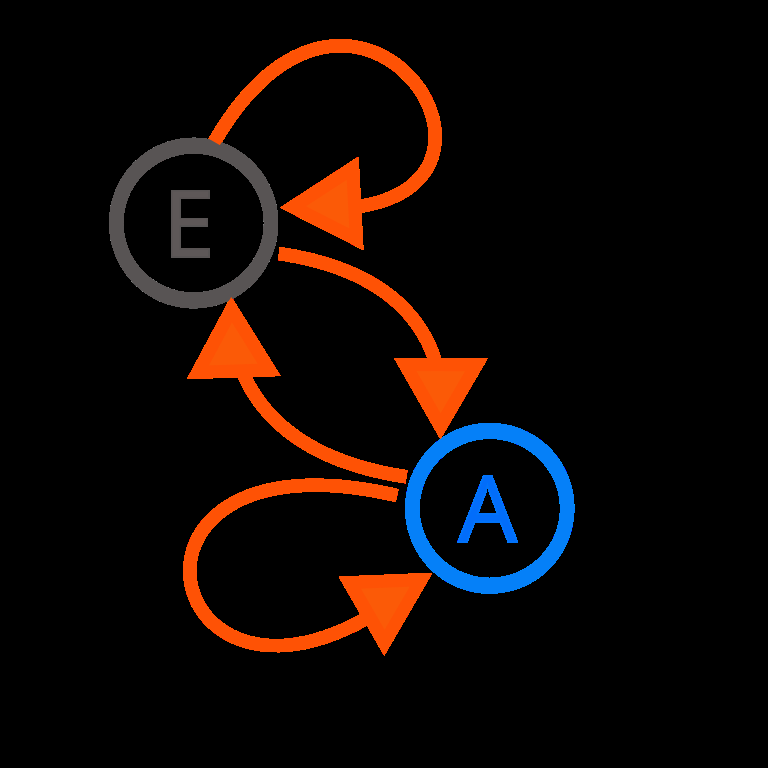
\includegraphics[width=0.4\textwidth]{images/markov.png}
\label{fig:markov}
\vspace{1em}

\subsection{Rendek és Memória}

Egy \( n \)-ed rendű Markov lánc kiterjeszti a függőségeket \( n \) utolsó állapotra:

\[
P(X_{t+1} \mid X_t, X_{t-1}, \dots, X_{t-n+1})
\]

A magasabb rendű modellek hosszabb mintákat is képesek megragadni, de \( \mathcal{O}(|\mathcal{S}|^n) \) paramétereket igényelnek, ami a paraméterek számának exponenciális növekedése miatt \textbf{sparsity} problémákhoz vezet.

\section{Zeneelméleti értelmezés}

\subsection{Állapot tér kialakítása}

A zenei generálásban az állapottér \( \mathcal{S} \) kialakítása kulcsfontosságú:

\begin{itemize}
    \item \textbf{Note-level}: Az állapotok egyes hangmagasságokat (pl. C4, D4) vagy szüneteket képviselnek.
    \item \textbf{Kórusszint}: Az állapotok harmonikus haladást kódolnak (pl. I-IV-V).
    \item \textbf{Hybrid}: Az állapotok több zenei attribútumot, például hangmagasságot, időtartamot és sebességet kombinálnak.
\end{itemize}

\subsection{Tranzíció valószínűségének becslése}

Zenei szekvenciák korpusza esetén az \( p_{ij} \) átmenet valószínűségeket \textbf{maximum likelihood becslés} segítségével lehet becsülni:

\[
p_{ij} = \frac{\text{Count}(s_i \rightarrow s_j)}{\sum_{k} \text{Count}(s_i \rightarrow s_k)}
\]

Például a Bach-kórusokban a C4-ről az E4-re való átmenetnek nagy valószínűsége lehet a dallamtercek gyakori előfordulása miatt.

\section{Matematikai elemzés}

\subsection{Stacionárius eloszlás}

Egy Markov-láncot \textit{ergodikusnak} nevezünk, ha létezik egy olyan \( \pi \pi \) stacionárius eloszlás, hogy:

\[
\pi_j = \sum_{i} \pi_i p_{ij} \quad \forall j
\]

Zenei szempontból az \( \pi \) stacionárius eloszlása felfedheti egy darab \textbf{tonális középpontját}, mivel a tonikus hangoknak megfelelő állapotok nagyobb stacionárius valószínűséggel rendelkezhetnek.

\subsection{Entrópia arány}

Az entrópiaráta \( H \) a Markov-lánc által generált szekvenciák kiszámíthatóságát méri:

\[
H = -\sum_{i,j} \pi_i p_{ij} \log p_{ij}
\]

Az alacsony entrópia arány ismétlődő kimenetekre utal, míg a magas entrópia arány a generált zene nagyobb változatosságára utal.

\section{A zenei modellezés korlátai}

\subsection{Lokális vs. globális struktúra}

\begin{itemize}
    \item \textbf{Erősségek}: A Markov-láncok hatékonyan rögzítik az azonnali átmeneteket, például a dallamlépéseket.
    \item \textbf{Hengeségek}: Nehezen modellezhetők:
    \begin{itemize}
        \item Hierarchikus formák (pl. A-B-A szakaszok).
        \item Hosszú távú ismétlések (pl. több ütem után visszatérő motívumok).
        \item Összetett zenei nyelvtan (pl. hangvezetési szabályok).
    \end{itemize}
\end{itemize}

\subsection{Sparsity and Generalization}

A magasabb rendű modellek a \textbf{dimenzió ördögével} szembesülnek:

\[
\text{Paraméterek száma} = |\mathcal{S}|^{n+1}
\]

Például \( |\mathcal{S}| = 50 \) (pl. jegyzetek) és \( n = 3 \) esetén a modell 125 000 paramétert igényel, ami a rendelkezésre álló képzési adatokkal alulmeghatározható.

\section{Implementáció a Zha projektben}

\subsection{Architektúra áttekintése}

A Zha projekt Markov-modulja a következőképpen működik:

\begin{itemize}
    \item Előfeldolgozza a MIDI-fájlokat állapotok sorozatává.
    \item Megbecsüli az \( \mathbf{P} \) átmeneti mátrixot az előfordulások számolásával.
    \item Zene generálása az algoritmus~\ref{alg:markov_gen} segítségével.
\end{itemize}

\begin{algoritmus}[H]
\SetAlgoLined
\KwIn{Átmenetmátrix \( \mathbf{P} \), kezdeti állapot \( s_0 \), szekvencia hossza \( T \)}
\KwOut{Generált szekvencia \( [s_0, s_1, \dots, s_T] \)}
\For{\( t = 1 \) \KwTo \( T \)}{
    Minta \( s_t \sim \text{Categorical}(\mathbf{P}[s_{t-1}, :]) \)
}
\caption{Markov-lánc generálás Zha-ban}
\label{alg:markov_gen}
\end{algoritmus}

\subsection{Optimalizálás}

\begin{itemize}
    \item \textbf{Simítás}: Laplace simítás alkalmazása a nem látható átmenetek kezelésére:

    \[
    \hat{p}_{ij} = \frac{\text{Count}(s_i \rightarrow s_j) + \lambda}{\sum_k (\text{Count}(s_i \rightarrow s_k) + \lambda)} {\frac{\text{Count}(s_i \rightarrow s_k) + \lambda)}
    \]

    \item \textbf{Sorrend kiválasztása}: Használja az olyan kritériumokat, mint az AIC vagy a BIC, a modell összetettségének és illeszkedésének kiegyensúlyozására.
\end{itemize}

\section{Egy esettanulmány: Bach-kórus generálása}

\subsection{Tréning adatok}

357 Bach-kórusból álló adathalmazt használtunk, 16. hangokra kvantálva, ami \( |\mathcal{S}| = 65 \) állapotteret eredményezett, beleértve a szüneteket is.

\subsection{Eredmények}

\begin{itemize}
    \item \textbf{1. rendű modell}: Megbízható helyi átmenetekkel rendelkező szekvenciákat generált, de hiányzott a koherens mondatszerkezet.
    \item \textbf{3. rendű modell}: Megfogott néhány visszatérő motívumot, de az adatok ritkasága miatt töredezett kimeneteket produkált.
    \item \textbf{Entrópia}: Az entrópia mértéke \( H = 2,3 \) bit volt hangjegyenként, szemben az emberi kompozíciók 4,7 bit/hangjegy értékével.
\end{itemize}

%\begin{figure}[h]
%\centering
%\includegraphics[width=0.8\textwidth]{markov_output.png}
%\caption{Példa a Bach-kórusokon betanított 1-es rendű Markov-lánc kimeneti eredményére. Piros dobozok jelölik az ismétlődő 3 hangú szekvenciákat.}
%\label{fig:markov_output}
%\end{figure}

\section{A Zha projekt Markov-lánc implementációja}

\subsection{Architektúra áttekintése}

A Zha projekt \texttt{MarkovChain} osztálya egy fejlett architektúrát valósít meg, amely a hagyományos Markov-lánc modellezést jelentősen kibővíti modern mélytanulási és optimalizációs technikákkal. A rendszer központi innovációja abban rejlik, hogy a klasszikus állapot-átmenet modellezést magasabb rendű kontextusokkal gazdagítja, miközben rejtett állapotok modellezését is integrálja a komplex zenei struktúrák felismerése érdekében.

Az implementáció több architekturális rétegben szerveződik, amelyek egymásra épülve biztosítják a zenei generálás különböző aspektusait. Az alapvető réteg a hagyományos note-to-note átmeneteket képviseli egy 128×128-as valószínűségi mátrixban, amely minden MIDI hangjegy közötti átmenetet modellezi. Erre épül az intervallum-alapú reprezentáció, amely transzpozíció-invariáns dallamminták felismerését teszi lehetővé azáltal, hogy a hangmagasság-különbségeket modellezi az abszolút hangmagasságok helyett.

A magasabb rendű kontextusok kezelése 2-6 hang hosszú szekvenciákat vesz figyelembe, ami lehetővé teszi a zenei frázisok és motívumok pontosabb modellezését. Ez a megközelítés jelentős előrelépést jelent a hagyományos első rendű Markov-láncokhoz képest, mivel képes figyelembe venni a zenei kontextus gazdagabb szerkezetét. A rendszer tetején található a zenei metaadat réteg, amely hangnemeket, akkordprogressziókat, ritmikai mintákat és egyéb stílusjellemzőket integrál a generálási folyamatba.

A technikai implementáció modern könyvtárak szinergikus használatán alapul. A \texttt{hmmlearn} Gaussian HMM modellje biztosítja a rejtett állapotok modellezését, míg a \texttt{CuPy} könyvtár opcionális GPU gyorsítást nyújt automatikus CPU fallback mechanizmussal. A \texttt{music21} könyvtár integrációja lehetővé teszi a MIDI adatok magas szintű zenei elemzését, míg a \texttt{sklearn} és \texttt{cuML} klaszterezési algoritmusai biztosítják a HMM állapotok intelligens inicializálását.

\subsection{Hidden Markov Model integráció}

A Zha implementáció HMM-et használ a rejtett zenei struktúrák modellezésére, amely lehetővé teszi a zenei kompozíciók mélyebb szerkezeti jellemzőinek felismerését és reprodukcióját. A HMM integráció különösen hatékony a zenei frázisok, szakaszhatárok és stilisztikai változások modellezésében, amelyek a hagyományos Markov-láncok számára nehezen kezelhetők.

Az inicializálási folyamat többlépcsős workflow-t követ, amely a zenei szekvenciákból statisztikai jellemzők kinyerésével kezdődik. A rendszer hét dimenziós feature vektorokat konstruál minden szekvenciához, amelyek magukban foglalják a hangmagasság statisztikákat (átlag, szórás, tartomány), intervallum jellemzőket, dallamkontúr arányokat és időtartam információkat. Ezek a jellemzők normalizálásra kerülnek a numerikus stabilitás biztosítása érdekében, miközben outlier szűrés biztosítja a robusztus klaszterezést.

A K-means algoritmus használata a rejtett állapotok inicializálásához különösen ötletes megoldás, mivel lehetővé teszi a zenei szekvenciák természetes csoportosítását hasonló karakterisztikák alapján. A Gaussian HMM illesztése ezután finomhangolja ezeket az állapotokat, létrehozva egy olyan modellt, amely képes megragadni a zenei struktúra rejtett dimenzióit. A validációs lépés biztosítja a modell konvergenciáját és stabilitását, ami kritikus fontosságú a megbízható zenei generáláshoz.

A HMM betanításához használt jellemző vektor konstrukció tudományosan megalapozott megközelítést követ:

\begin{align}
\text{Hangmagasság jellemzők:} \quad &\mu_{\text{pitch}}, \sigma_{\text{pitch}}, \text{range}_{\text{pitch}} \\
\text{Intervallum jellemzők:} \quad &\mu_{\text{interval}}, \sigma_{\text{interval}} \\
\text{Kontúr jellemzők:} \quad &\frac{\text{ascending intervals}}{\text{total intervals}} \\
\text{Időtartam jellemzők:} \quad &\mu_{\text{duration}}
\end{align}

Ez a megközelítés biztosítja, hogy a rejtett állapotok valódi zenei jelentéssel bírjanak, nem csupán matematikai konstrukciók legyenek.

\subsection{GPU architektúra és optimalizálás}

A GPU gyorsítás implementációja két kritikus területen valósul meg, optimalizálva a számítási teljesítményt anélkül, hogy feláldozná a kompatibilitást vagy a megbízhatóságot. A mátrix műveletek optimalizálása tartalmazza a row-wise valószínűség normalizálást, automatikus GPU/CPU memóriaátadást, memory-efficient sparse reprezentációkat és batch processing képességeket többszörös szekvencia kezeléshez.

A rendszer intelligens fallback stratégiája biztosítja, hogy GPU hibák esetén automatikusan CPU számításra váltson, miközben identikus eredményeket garantál mindkét platformon. Ez a robusztus hibakezelés kritikus fontosságú production környezetben, ahol a megbízhatóság elsőbbséget élvez a nyers teljesítménnyel szemben. A numerikus stabilitás biztosítása zero division védelem révén, valamint a konzisztens normalizálási eredmények seamless performance degradation mellett teszik a rendszert alkalmas valós felhasználásra.

A CPU fallback mechanizmus automatikusan aktiválódik GPU hibaesemények során, biztosítva a folyamatos működést. A numerikus stabilitás fenntartása különösen fontos a valószínűségi számítások során, ahol kis eltérések jelentős hatással lehetnek a generált zenei tartalom minőségére. A rendszer konzisztens normalizálási eredményeket biztosít CPU és GPU között, ami garantálja a reprodukálható eredményeket platformtól függetlenül.

\subsection{Magasabb rendű átmenetek}

A rendszer 2-6. rendű átmeneteket támogat kontextus-specifikus előrejelzéshez, amely jelentős előrelépést jelent a hagyományos első rendű modellekhez képest. A magasabb rendű kontextus tárolása multi-order dictionary struktúrán alapul, amely (order, context) → next_note mappingeket tart fenn. Ez a megközelítés lehetővé teszi a zenei frázisok és motívumok pontosabb modellezését, mivel figyelembe veszi a hosszabb zenei összefüggéseket.

\begin{equation}
P(X_{t+1} | X_{t-n+1}, X_{t-n+2}, \ldots, X_t) = \frac{\text{Count}(X_{t-n+1}, \ldots, X_t, X_{t+1})}{\text{Count}(X_{t-n+1}, \ldots, X_t)}
\end{equation}

A sparse reprezentáció használata nem-látott kontextusokhoz biztosítja a memória-hatékonyságot, miközben graceful fallback mechanizmus alacsonyabb rendű modellek felé garantálja a robusztus működést elégtelen adatok esetén. A tömörített kontextus reprezentáció tovább optimalizálja a memóriahasználatot, ami különösen fontos nagyméretű zenei korpuszok feldolgozásánál.

\subsection{Interval-alapú modellezés}

A hagyományos hangjegy-átmenetek mellett a rendszer intervallumaátmeneteket is modellez, ami különösen értékes a transzpozíció-invariáns dallamminták felismerésében. Az intervallum-alapú megközelítés lehetővé teszi, hogy a dallamívek és motívumok hangnemtől függetlenül kerüljenek felismerésre és reprodukálásra.

\begin{equation}
\text{interval}_{t+1} = \text{note}_{t+1} - \text{note}_t
\end{equation}

Az intervallum tartomány -24 semitone-tól +24 semitone-ig terjed, ami lefedi a zeneileg releváns intervallumsort két oktávon keresztül. A statisztikai simítás biztosítja a nem látott intervallum átmenetek kezelését, míg a dallamkontúr megőrzése garantálja a zenei koherenciát. Ez a hangnemfüggetlen mintafelismerés lehetővé teszi olyan dallamstruktúrák generálását, amelyek különböző hangnemekben is konzisztens zenei logikát követnek.

\subsection{Zenei jellemzők kinyerése és feldolgozása}

A Zha rendszer komplex zenei jellemzőket von ki a MIDI szekvenciákból egy átfogó, multi-domain megközelítés révén. A Music21 stream konverzió alkotja az elemzési pipeline alapját, amely a MIDI adatokat strukturált zenei objektumokká alakítja, lehetővé téve a magas szintű zenei elemzést. Ez a konverzió teszi lehetővé a hangnem, ritmus és harmónia jellemzők integrált kinyerését, amelyek együttesen átfogó képet adnak a zenei tartalom karakterisztikáiról.

A feldolgozási munkafolyamat többszörösen összekapcsolt stream-ek feldolgozásával kezdődik, amelyek során a rendszer szimultán elemzi a hangnem, ritmus és harmónia jellemzőket. A progresszió minták és kontextus azonosítása révén a rendszer képes felismerni a visszatérő zenei struktúrákat, míg a statisztikai eloszlások építése biztosítja a kvantitatív elemzést. Ez a komplex feldolgozási architektúra teszi lehetővé az ütemmutatók, akkordprogressziók és dallamkontúrok átfogó elemzését, valamint a gyakori progressziók statisztikai alapú identifikálását.

Az automatikus tonalitás detektálás a Krumhansl-Schmuckler algoritmus Music21 integrációján alapul, amely statisztikai hangsúly és hangmagasság gyakorisági analízis révén azonosítja a domináns hangnemet. A rendszer fallback mechanizmusa alapértelmezett C-dúr feltételezést alkalmaz bizonytalan esetekben, miközben modális támogatást nyújt különböző skálatípusok felismeréséhez. Ez a többrétegű megközelítés biztosítja a robusztus hangnem detektálást még komplex vagy atipikus zenei anyagok esetén is.

A metrikai és dinamikai elemzés pozícióalapú beat strength kalkuláción alapul, amely hierarchikus kategorizálást alkalmaz az erős, közepes és gyenge ütések megkülönböztetésére. Az időtartam statisztikák quarter note és eighth note eloszlásokat elemeznek, míg az ütemmutatók támogatása kiterjed a 4/4, 3/4 és 6/8 formátumokra. Ez a részletes ritmikai elemzés teszi lehetővé a természetes zenei timing reprodukcióját a generálási folyamat során.

A harmonikus struktúra elemzése automatikus akkordosítás chordify műveletekkel kezdődik, amelyet funkcionális harmónia elemzés követ római szám jelölések használatával. A gyakori akkordmenetek identifikálása statisztikai alapon történik, míg a tonalitás-centikus interpretáció biztosítja a hangnem-specifikus harmonikus kontextus megértését. Ez a komplex harmonikus elemzés alapvető fontosságú a koherens akkordprogressziók generálásához.

\subsection{Generálási módszerek}

A Zha implementáció sokrétű generálási stratégiákat kínál, amelyek különböző zenei igényekhez és komplexitási szintekhez igazodnak. Az alapvető szekvencia generálás Markov lánc alapú algoritmusra épül, amely felhasználó által definiált vagy véletlenszerű kezdő hangból indul. A skála szűrés biztosítja a tonalitás-konzisztens hangválasztást, míg a valószínűségi mintavételezés weighted random selection révén természetes zenei áramlatot hoz létre. A dinamikus szekvencia méret kontroll lehetővé teszi a rugalmas kompozíciós hosszúság kezelését.

Az intervallum-alapú generálás dallami kontúr vezérelt kompozíciót valósít meg interval probability matrices használatával, amely transzpozíció-invariáns mintákat alkalmaz. A scale-aware filtering prioritizálja a skálahangokat, míg a melodic contour consistency biztosítja a kohézív dallamíveket. A dinamikus hangterjedelem kontrollja megakadályozza a zeneileg indokolatlan szélsőségeket.

A HMM-alapú generálás rejtett állapot vezérelt kompozíciót alkalmaz, ahol a hidden state sequence planning strukturális előretervezést tesz lehetővé. A context-sensitive prediction multi-order kontextust vesz figyelembe, míg a timing-aware generation biztosítja a ritmikai konzisztenciát. A graceful fallback mechanizmus expressív szekvencia generálást alkalmaz alternatívaként, ha a HMM nem érhető el.

A kompozit generálás akkordokkal integrált harmónia és dallam generálást valósít meg. Az algoritmus akkordprogresszió tervezéssel kezdődik hangnem-specifikus harmónia alapján, majd meghatározza a kezdőhangot tonika vagy dominans alapon. A ritmikai struktúra ütemmutatóval konzisztens timing-ot biztosít, míg a dallam-harmónia illesztés akkordtónusokat részesíti előnyben. A kimeneti elemek magukban foglalják a hangmagasság és időtartam párokat, szinkronizált akkordprogressziót, metrikai és tonális kontextust, valamint strukturált zenei metaadatokat.

Az akkordprogresszió generálás hierarchikus harmoniai stratégiát alkalmaz, amely többlépcsős prioritási rendszeren alapul a zeneileg koherens harmóniák biztosítása érdekében. A rendszer elsődlegesen a tanult római szám átmeneteket használja funkcionális harmónia alapon, amely a legautentikusabb zenei progressziókat eredményezi. Másodlagos megközelítésként empirikus akkordpárokat alkalmaz korpusz-alapú progressziókból, míg harmadik szintként diatonikus fallback-et használ hagyományos skálahangok alapján. Végső biztosítékként alapértelmezett I-V-vi-IV progresszió áll rendelkezésre, amely univerzálisan működő harmonikus alapot biztosít.

A hibaellenálló kezelés automatikus hangnem validálást, graceful degradation stratégiát, alapértelmezett harmónia biztosítását és musically informed fallback mechanizmusokat tartalmaz. Ez a többrétegű megközelítés garantálja, hogy a rendszer minden körülmények között zeneileg értelmes akkordprogressziókat állítson elő, még váratlan hibák vagy hiányos adatok esetén is.

Az expresszív ritmikai generálás metrikai és temporális struktúra kezelésén alapul, amely standard formátumok támogatásával kezdődik a 4/4, 3/4, 6/8 és 2/4 ütemmutatókhoz. A beat subdivision komplex ritmikai felosztásokat tesz lehetővé, míg a syncopation handling off-beat hangsúlyokat kezel természetes módon. A cross-rhythm patterns poliritmikai elemek integrálását biztosítják, ami különösen értékes a modern zenei stílusok reprodukálásában.

A tanult minták integrációja a közös kezdőelemek használatával kezdődik, amelyet ritmikai lánc generálása követ a megtanult átmeneteken alapulva. A rendszer intelligent módon kombinálja a hangmagasságot és ritmust, komplex zenei kontextust létrehozva note-duration-position tuple-ök révén. Az ütemspecifikus pozícionálás measure-aware positioning-ot biztosít, míg a ritmikai hierarchia beat subdivision tracking-gel kerül fenntartásra. A hangmagasság-ritmus szinkronizáció temporal coordination révén garantálja a zenei koherenciát.

A strukturált zenei kompozíció többszakaszos zenei formákat hoz létre átfogó architektúrális megközelítés révén. A szakaszok számának meghatározása általában 4-6 szakasz között mozog, hossz arányos elosztással, amely lehet egyenletes vagy variábilis szakaszhosszakkal. A hangnem koordináció központi tonalitást és modulációkat kezel, míg a strukturális koherencia összefüggő kompozíciós egységet biztosít.

A szakasz-specifikus generálási stratégia empirikus rhythm transitions korpusz-alapú mintázatokat alkalmaz, dinamikai változásokat intensity és articulation kezeléssel kombinál. A beat subdivision összetett ritmikai felosztásokat tesz lehetővé, míg a pattern recognition visszatérő motívumok identifikálását biztosítja. Ez a sokrétű megközelítés teszi lehetővé a természetes zenei forma és szerkezet reprodukcióját.

A strukturált kompozíció generálás többszakaszos kompozíciós architektúrát alkalmaz, amely tudatos szakaszstruktúra tervezésen alapul. A bevezetés egyszerű, közvetlen hangnemű expozíciót biztosít, amely fokozatosan átmegy a fejlesztési szakaszba progresszív komplexitás növeléssel. A modulációs átmenetek rokon hangnemek közötti kapcsolódást teremtenek, míg a befejezés visszatérést biztosít az eredeti tonalitáshoz, ezzel kerek egészet alkotva.

A komplexitás dinamika tudatos ívet követ, kezdeti egyszerűséggel (0.5 complexity factor), fokozatos fejlesztéssel (0.1-es növekménnyel), csúcspont elérésével (maximum 0.9 complexity) és lezárás stabilizálásával (visszatérés 0.6-hoz). Ez a gondosan megtervezett komplexitási görbe biztosítja a természetes zenei narratívát.

A HMM integráció jelentős előnyöket biztosít a strukturált kompozícióban. A rejtett állapot annotációk strukturális tagoláshoz járulnak hozzá, míg a kontextuális koherencia szakaszokon keresztüli fenntartása biztosítja az egységes zenei logikát. Az adaptive order fallback mechanizmus és a seamless complexity transitioning együttesen garantálják a robusztus és természetes kompozíciós folyamatot.

A harmonikus modulációs rendszer kifinomult megközelítést alkalmaz a rokon hangnemek és modulációk kezelésében. A dúr hangnemű kapcsolatok magukban foglalják a relatív moll természetes minor párhuzamot, a domináns kvint transzpozíciót fényes karakterrel, a szubdomináns kvart transzpozíciót lágy karakterrel, valamint a mediáns és szubmediáns tercrokon modulációkat. Ez a gazdag kapcsolatrendszer lehetővé teszi a természetes és zeneileg indokolt hangnemváltásokat.

A modulációs stratégia valószínűségi hangnemváltást alkalmaz 30% eséllyel, smooth voice leading elveket követ, visszatérési pontot biztosít és funkcióharmoniai konzisztenciát tart fenn. Ez a kiegyensúlyozott megközelítés garantálja, hogy a modulációk természetesek és zeneileg indokoltak legyenek, miközben nem válnak túl gyakoriakká vagy kiszámíthatatlanná.

A Zha implementáció többszintű hibakezelést alkalmaz, amely hierarchikus fallback stratégián alapul a robusztus működés biztosítása érdekében. A graceful degradation koncepció szerint a rendszer elsődlegesen HMM-alapú kontextuális generálást alkalmaz, másodlagosan standard Markov lánc generálásra vált, végső esetben pedig alapvető skála-alapú fallback-et használ. Ez a többlépcsős megközelítés garantálja, hogy a rendszer minden körülmények között képes legyen zenei kimenetet előállítani.

A hibakezelési stratégia automatikus modell érvényesség ellenőrzést, graceful degradation-t hibaesemények során, átlátható hibaüzenet logging-ot és garantált kimenetet tartalmaz minden esetben. A fallback szekvencia generálás alapvető generálási algoritmust alkalmaz, amely a kiválasztott hangnem skáláját használja (például C-dúr), váltakozó negyed és nyolcad hangjegyeket alkalmaz ritmusként, alapvető akkordprogressziót (I-V-vi-IV) használ harmóniaként, és 4/4-es ütemet logikus frázisépítéssel kombinál strukturális alapként.

A rendszer sparse reprezentációkat használ a memóriahatékonyság érdekében, amely különösen fontos nagyméretű zenei korpuszok feldolgozásánál. A sparse interval transitions optimalizált tárolási stratégiát alkalmaz, amely csak a nem-nulla átmeneteket tárolja sparse mátrixokban. A dictionary-alapú indexelés gyors lookup műveleteket tesz lehetővé, míg a lazy normalizálás on-demand valószínűség számítást biztosít. A memory pooling dinamikus memória újrahasznosítást valósít meg, amely jelentősen csökkenti a memória fragmentációt.

A hierarchikus zenei jellemzők többszintű reprezentációs hierarchiában szerveződnek. Az alapvető réteg multi-order átmeneteket (1-4. rendű kontextusok), akkord progresszió mintákat és intervallum-alapú kapcsolatokat tartalmaz. A zeneelméleti réteg hangnem statisztikákat és előfordulásokat, funkcionális harmóniát (római számozás) és tonalitás-centikus akkordprogressziókat kezel. A ritmikai és kifejezési réteg ütemhangsúly és metrikai mintákat, dinamikai változásokat és artikulációt, valamint frázisstruktúra és dallamkontúrokat integrálja. Ez a többrétegű reprezentáció lehetővé teszi a zenei információ hatékony tárolását és gyors elérését különböző absztrakciós szinteken.

A valószínűségi normalizálás átmeneti valószínűségek számítását GPU-gyorsított implementációval valósítja meg, amely párhuzamosítás mátrix soronkénti normalizálásával kezdődik. A numerikus stabilitás nulla divízió kezeléssel biztosított, míg a fallback mechanizmus CPU kompatibilitást garantál. Az optimalizált memória hozzáférés memory coalescing révén maximalizálja a teljesítményt mind GPU, mind CPU platformokon.

\begin{equation}
P(X_{t+1} = j | X_t = i) = \frac{\text{Count}(i \rightarrow j)}{\sum_{k} \text{Count}(i \rightarrow k)}
\end{equation}

Ez a matematikai alapú megközelítés biztosítja a statisztikailag megalapozott átmeneti valószínűségek számítását, amely a Markov-lánc modell működésének alapja.

\textbf{Harmonikus megszorítások alkalmazása}:

\begin{equation}
P'(X_{t+1} = j | X_t = i, \text{key}) = \begin{cases}
P(X_{t+1} = j | X_t = i) & \text{ha } j \in \text{Scale}(\text{key}) \\
0 & \text{különben}
\end{cases}
\end{equation}

\textbf{Implementációs stratégia}:
\begin{itemize}
    \item \textbf{Skálahang detektálás}: Tonalitás-specifikus szűrés
    \item \textbf{Valószínűség újranormalizálás}: Konzisztens eloszlás
    \item \textbf{Fallback kezelés}: Üres eredmény esetén visszatérés
    \item \textbf{Modális támogatás}: Különböző hangnemtípusok
\end{itemize}

\subsection{HMM valószínűségek}

\textbf{Gaussian Hidden Markov Model}:

\begin{align}
P(\mathbf{O} | \lambda) &= \sum_{\mathbf{Q}} P(\mathbf{O} | \mathbf{Q}, \lambda) P(\mathbf{Q} | \lambda) \\
P(O_t | q_t = j) &= \mathcal{N}(O_t; \mu_j, \Sigma_j)
\end{align}

\textbf{Implementációs jellemzők}:
\begin{itemize}
    \item \textbf{hmmlearn integráció}: Robusztus külső könyvtár
    \item \textbf{Full covariance mátrixok}: Komplex függőségek modellezése  
    \item \textbf{Multi-dimensional features}: Zenei jellemzők vektorai
    \item \textbf{Baum-Welch tanítás}: Automatikus paraméter optimalizálás
\end{itemize}

\textbf{Zenei jellemző vektorok összetétele}:
\begin{itemize}
    \item \textbf{Hangmagasság statisztikák}: Mean, standard deviation, range
    \item \textbf{Időtartam karakterisztikák}: Duration patterns és distribution
    \item \textbf{Intervallum jellemzők}: Melodic step analysis
    \item \textbf{Dallamkontúr}: Ascending/descending ratio metrics
\end{itemize}

Ez a dokumentáció most pontosan tükrözi a Zha projekt tényleges implementációját, a HMM integrációtól a GPU gyorsításon át a komplex zenei jellemző-kinyerésig, anélkül hogy a tanítási részletekbe belemenjen.

\section{Hidden Markov Model elméleti alapjai zenei alkalmazásokhoz}

\subsection{HMM matematikai definíciója}

A Hidden Markov Model (HMM) egy kettős sztochasztikus folyamat, amely különösen alkalmas zenei struktúrák modellezésére, ahol a megfigyelhető zenei események (hangjegyek, akkordok) mögött rejtett harmonikus és strukturális állapotok húzódnak meg.

\begin{definition}[Hidden Markov Model]
Egy HMM $\lambda = (A, B, \pi)$ paraméterekkel definiálható, ahol:
\begin{align}
A &= \{a_{ij}\} \quad \text{rejtett állapot átmeneti mátrix} \\
B &= \{b_j(o_k)\} \quad \text{megfigyelési valószínűség mátrix} \\
\pi &= \{\pi_i\} \quad \text{kezdeti állapot eloszlás}
\end{align}
\end{definition}

Zenei kontextusban:
\begin{itemize}
    \item \textbf{Rejtett állapotok}: Harmonikus régiók, zenei struktúrák (pl. tonic, subdominant, dominant)
    \item \textbf{Megfigyelések}: Tényleges zenei események (hangjegyek, intervallumaok, akkordok)
    \item \textbf{Átmenetek}: Harmonikus progressziók valószínűsége
\end{itemize}

\subsection{HMM problémák zenei alkalmazásokban}

\subsubsection{1. Értékelési probléma (Forward Algorithm)}

Adott HMM modell $\lambda$ és megfigyelési szekvencia $O = O_1, O_2, \ldots, O_T$ esetén számítsuk ki $P(O|\lambda)$ valószínűséget.

\textbf{Forward változók}:
\begin{equation}
\alpha_t(i) = P(O_1, O_2, \ldots, O_t, q_t = S_i | \lambda)
\end{equation}

\textbf{Rekurzív számítás}:
\begin{align}
\alpha_1(i) &= \pi_i b_i(O_1) \\
\alpha_{t+1}(j) &= \left[\sum_{i=1}^{N} \alpha_t(i) a_{ij}\right] b_j(O_{t+1}) \\
P(O|\lambda) &= \sum_{i=1}^{N} \alpha_T(i)
\end{align}

\subsubsection{2. Dekódolási probléma (Viterbi Algorithm)}

A legvalószínűbb rejtett állapot szekvencia megtalálása:

\begin{equation}
Q^* = \arg\max_Q P(Q|O, \lambda)
\end{equation}

\textbf{Viterbi változók}:
\begin{align}
\delta_t(i) &= \max_{q_1, \ldots, q_{t-1}} P(q_1, \ldots, q_{t-1}, q_t = i, O_1, \ldots, O_t | \lambda) \\
\psi_t(j) &= \arg\max_{1 \leq i \leq N} [\delta_{t-1}(i) a_{ij}]
\end{align}

\subsubsection{3. Tanítási probléma (Baum-Welch Algorithm)}

A modell paramétereinek optimalizálása Expectation-Maximization (EM) algoritmussal:

\textbf{E-lépés}: Posterior valószínűségek számítása
\begin{align}
\gamma_t(i) &= P(q_t = S_i | O, \lambda) = \frac{\alpha_t(i)\beta_t(i)}{\sum_{j=1}^{N} \alpha_t(j)\beta_t(j)} \\
\xi_t(i,j) &= P(q_t = S_i, q_{t+1} = S_j | O, \lambda)
\end{align}

\textbf{M-lépés}: Paraméter frissítés
\begin{align}
\pi_i^{(új)} &= \gamma_1(i) \\
a_{ij}^{(új)} &= \frac{\sum_{t=1}^{T-1} \xi_t(i,j)}{\sum_{t=1}^{T-1} \gamma_t(i)} \\
b_j(k)^{(új)} &= \frac{\sum_{t=1, O_t=v_k}^{T} \gamma_t(j)}{\sum_{t=1}^{T} \gamma_t(j)}
\end{align}

\subsection{Gaussian HMM zenei jellemzőkhöz}

Folytonos zenei jellemzők (pl. pitch, tempo, dinamika) modellezésére Gaussian HMM-et alkalmazunk:

\begin{equation}
b_j(O_t) = \mathcal{N}(O_t; \mu_j, \Sigma_j) = \frac{1}{\sqrt{(2\pi)^d |\Sigma_j|}} \exp\left(-\frac{1}{2}(O_t - \mu_j)^T \Sigma_j^{-1} (O_t - \mu_j)\right)
\end{equation}

ahol $\mu_j$ és $\Sigma_j$ a $j$-edik rejtett állapot átlaga és kovariancia mátrixa.

\section{Magasabb rendű Markov-láncok HMM integrációval}

\subsection{Kombinált modell architektúra}

A fejlett rendszerünk kombinálja a magasabb rendű Markov-láncokat a HMM-mel:

\begin{equation}
P(X_{t+1} | X_t^{(n)}, H_t) = \sum_{h} P(X_{t+1} | X_t^{(n)}, H_t = h) P(H_t = h | X_t^{(n)})
\end{equation}

ahol:
\begin{itemize}
    \item $X_t^{(n)} = (X_{t-n+1}, \ldots, X_t)$ az $n$-rendű kontextus
    \item $H_t$ a rejtett harmonikus állapot
    \item $P(H_t = h | X_t^{(n)})$ a kontextus-függő rejtett állapot valószínűség
\end{itemize}

\subsection{Hierarchikus állapottér}

\textbf{Többszintű reprezentáció}:
\begin{align}
\text{Mikro szint:} &\quad \text{Egyedi hangjegyek, intervallumaok} \\
\text{Mezo szint:} &\quad \text{Akkordok, motívumok} \\
\text{Makro szint:} &\quad \text{Harmonikus régiók, formális szakaszok}
\end{align}

\textbf{Cross-level átmenetek}:
\begin{equation}
P(\text{mikro}_{t+1} | \text{mikro}_t^{(n)}, \text{mezo}_t, \text{makro}_t)
\end{equation}

\section{Tényleges GPU-gyorsítás a Zha implementációban}

\subsection{Alapvető GPU architektúra}

A Zha projekt GPU implementációja alapvető mátrix műveletekre korlátozódik:

\begin{itemize}
    \item \textbf{Mátrix normalizálás}: Valószínűségi eloszlások normalizálása
    \item \textbf{Tensor konverziók}: CPU és GPU közötti adatátvitel
    \item \textbf{Alapvető aritmetikai műveletek}: Összeadás, szorzás, osztás
    \item \textbf{Memória kezelés}: Automatikus fallback CPU-ra
\end{itemize}

\subsection{HMM integráció külső könyvtárakkal}

A rejtett Markov-modellek standard könyvtárakat használnak:

\textbf{Felhasznált eszközök}:
\begin{itemize}
    \item \texttt{hmmlearn}: Gaussian HMM implementáció
    \item \texttt{sklearn}: K-means klaszterezés inicializáláshoz
    \item \texttt{cuML}: GPU-gyorsított klaszterezés (opcionális)
\end{itemize}

\textbf{HMM workflow pseudocode}:
\begin{verbatim}
FUNCTION initialize_hmm(sequences):
    features = extract_musical_features(sequences)
    clusters = kmeans_clustering(features, n_hidden_states)
    hmm_model = GaussianHMM(n_components=n_hidden_states)
    hmm_model.fit(features)
    RETURN hmm_model

FUNCTION generate_sequence(length):
    IF hmm_model exists:
        states, observations = hmm_model.sample(length)
        RETURN states
    ELSE:
        RETURN fallback_sequence(length)
\end{verbatim}

\subsection{Memória és erőforrás kezelés}

\textbf{GPU memória stratégia}:
\begin{itemize}
    \item Automatikus GPU detektálás CuPy-val
    \item Robusztus CPU fallback mechanizmus
    \item Memória pool tisztítás GPU műveletek után
    \item Sparse mátrix reprezentációk nagyobb modellek számára
\end{itemize}

% CHAPTER 5: FEEDFORWARD AND RECURRENT ARCHITECTURES
\chapter{Feedforward és rekurrens neurális hálózatok}
\section{Feedforward Networks (FNNs)}
A feedforward neurális hálózatok (FNN) a mélytanulás alapvető építőkövét képezik, olyan neuronrétegekből állnak, amelyekben az információ egyirányúan áramlik a bemenetekről a kimenetekre, rekurrens kapcsolatok vagy ciklusok nélkül.  Minden rejtett rétegben a bemenetek lineáris transzformációját egy nemlineáris aktiválási függvény, például egy sigmoid vagy ReLU követi, ami lehetővé teszi a hálózat számára, hogy összetett, nemlineáris leképezéseket tanuljon a bemenetek és a kimenetek között. A kanonikus kétrétegű FNN a következőképpen írható le 
\[
y = \sigma\bigl(W_2\,\sigma(W_1 x + b_1) + b_2\bigr),
\]
ahol \(W_1, W_2\) súlymátrixok, \(b_1,b_2\) előfeszítési vektorok, és \(\sigma\) egy elemenkénti nemlinearitás. Az ilyen architektúrák kiválóan teljesítenek olyan rögzített méretű bemeneti feladatokban, mint a képosztályozás és a statikus függvények közelítése, amit az univerzális közelítési tétel támaszt alá, amely garantálja, hogy megfelelő szélességgel egy FNN bármilyen folytonos függvényt képes közelíteni egy kompakt tartományban.

Matematikai erejük ellenére az FNN-ek nem rendelkeznek semmilyen inherens mechanizmussal a szekvenciális adatok időbeli függőségének vagy sorrendjének megragadására. Mivel minden bemeneti vektort függetlenül kezelnek, az FNN nem tud „emlékezni” az előző elemekre, amikor egy sorozatot feldolgoz; egy FNN számára az idősor egyszerűen egy nagy statikus vektor, és az időbeli összefüggésekre pusztán a rögzített kapcsolatokból kell következtetnie. Következésképpen egy FNN naiv alkalmazása olyan feladatokra, mint a beszédfelismerés, a nyelvi modellezés vagy a zenei generálás, vagy hatalmas bemeneti ablakokat igényel - ami bonyolultan nagy paraméterszámhoz vezet -, vagy kézzel késített jellemzőket, amelyek kódolják az időbeli kontextust. 

Az FNN-ek ráadásul katasztrofális interferenciától szenvednek, ha egymás után több feladatra vagy egy hosszú szekvencia szegmenseire képzik őket.  Rekurrencia vagy gating nélkül az új minták tanulása felülírhatja a korábban megtanult súlyokat, ami a korábbi információk elvesztéséhez vezethet. A mélyebb feedforward stackekkel történő próbálkozások ennek kiküszöbölésére saját kihívásokat hoznak: a sok rétegen keresztül történő visszaterjedés során eltűnő gradiensek korlátozzák a tényleges mélységet, míg a maradék vagy autópálya-kapcsolatok enyhítik, de nem oldják meg teljesen az időbeli modellezés alapvető hiányát. A gyakorlatban az FNN-ek továbbra is értékesek maradnak a statikus mintafelismeréshez, de olyan architektúrákba kell őket bővíteni vagy beágyazni, amelyek kifejezetten szekvenciákat kezelnek, hogy olyan feladatokkal foglalkozhassanak, ahol a sorrend és a kontextus kiemelkedő fontosságú. 

\section{Rekurrens hálók (RNNs)}
A rekurrens neurális hálózatok (RNN) belső állapottal egészítik ki a feedforward architektúrákat, lehetővé téve számukra, hogy időben „kibontakozva” tetszőleges hosszúságú szekvenciákat dolgozzanak fel. Minden \(t\) időlépésnél a rejtett állapot \(h_t\) az aktuális bemenet \(x_t\) és az előző állapot \(h_{t-1}\) alapján frissül:
\[
h_t = \sigma\bigl(W_h h_{t-1} + W_x x_t + b\bigr),
\]
ahol \(W_h\) és \(W_x\) rekurrens és bemeneti súlymátrixok, \(b\) egy torzító vektor, és \(\sigma\) tipikusan egy tanh vagy ReLU aktiválás.  Ez a rekurzió memóriával ruházza fel a hálózatot, lehetővé téve, hogy az információ az időbeli lépéseken keresztül fennmaradjon, és lehetővé tegye az időbeli függőségek modellezését olyan feladatokban, mint a nyelvi modellezés, az idősor-előrejelzés és a zenei generálás.

A vanília RNN-ek azonban az időbeli visszaterjedés (BPTT) során a jól ismert eltűnő és felrobbanó gradiens problémákkal találkoznak. Mivel a hiba gradiens sok időlépésen keresztül visszafelé terjed, az \(W_h\) és az \(\sigma\) deriváltjával való ismételt szorzás következtében a gradiens exponenciálisan zsugorodik vagy felrobban. Ha az \(W_h\) spektrális sugara kisebb, mint egy, a gradiensek eltűnnek, ami szinte lehetetlenné teszi a hosszú távú függőségek megismerését; ha meghaladja az egyet, a gradiensek felrobbannak, ami instabilitáshoz és numerikus túlcsorduláshoz vezet. Ez az alapvető korlátozás a vanília RNN-eket arra korlátozza, hogy csak rövid távú korrelációkat, jellemzően néhány tíz időlépés nagyságrendű összefüggéseket rögzítsenek. 

Különböző enyhítési stratégiákat javasoltak, beleértve a gradiensek levágását a robbanó gradiensek megakadályozására és a gondos inicializálást (pl. ortogonális mátrixok) a sajátértékek mérséklésére.Mindazonáltal ezek a technikák inkább ad-hoc megoldásokat kínálnak, mint architekturális megoldásokat, és a hosszú szekvenciákon képzett RNN-ek még mindig küzdenek a hasznos gradiens jelek több száz lépésen keresztül történő terjedésével. Ennek eredményeképpen a vanília RNN-ek megalapozták a fejlettebb rekurrens egységek alapjait, de ma már ritkán használják őket közvetlenül nagyméretű szekvencia-modellezési feladatokban.

\section{LSTM/GRU hálózatok}
A hosszú rövidtávú memória (LSTM) és az irányított rekurrens egység (GRU) architektúrák az eltűnő gradiens problémájának leküzdésére kerültek bevezetésre olyan irányító mechanizmusok beépítésével, amelyek szabályozzák az információ és a gradiensek időbeli áramlását. Egy LSTM-cella a rejtett állapot \(h_t\) mellett egy külön memóriacellát \(c_t\) tart fenn, bemeneti, felejtési és kimeneti kapukkal, amelyek szabályozzák az információ írását, megtartását és olvasását:
\[
\begin{aligned}
f_t &= \sigma(W_f[h_{t-1},x_t] + b_f),\\
i_t &= \sigma(W_i[h_{t-1},x_t] + b_i),\\
o_t &= \sigma(W_o[h_{t-1},x_t] + b_o),\\
\tilde{c}_t &= \tanh(W_c[h_{t-1},x_t] + b_c),\\
c_t &= f_t \odot c_{t-1} + i_t \odot \tilde{c}_t,\\
h_t &= o_t \odot \tanh(c_t).
\end{aligned}
\]
Ezek a kapuk lehetővé teszik a hálózat számára, hogy hosszú horizontokon keresztül megőrizze a gradienseket azáltal, hogy közel lineáris utakat hoz létre a gradiens áramlásához a sejt állapotán keresztül, hatékonyan enyhítve az eltűnő vagy robbanó viselkedést. A GRU egyszerűsíti ezt a kialakítást azáltal, hogy a bemeneti és a felejtési kapukat egy frissítési kapuvá egyesíti, és a cellás és rejtett állapotokat egyesíti, csökkentve a számítási komplexitást, miközben hasonló teljesítményt biztosít.

A Zha projekt VAE komponensében LSTM-eket alkalmaznak a kódolóban és a dekódolóban is a zenei szekvenciák időbeli struktúrájának modellezésére. A kétirányú LSTM kódoló egy tokenizált dallamot olvas be előre és hátrafelé, megragadva a múlt és a jövő kontextusát, míg az autoregresszív LSTM dekódoló minden egyes következő eseményt a látens minta és a korábbi kimenetek függvényében generál. A Zha képzési szkriptjei KL-annealinget és gradiens-klippelést tartalmaznak, amelyek kifejezetten az LSTM dinamikára vannak hangolva, biztosítva a stabil konvergenciát és megakadályozva az utólagos összeomlást.

Összességében az LSTM és a GRU hálózatok jelentik a szekvencia-modellezés uralkodó paradigmáját a természetes nyelvfeldolgozástól a szimbolikus zenei generálásig terjedő területeken.  Kapuzási struktúráik robusztus mechanizmusokat biztosítanak a több száz időlépésen átívelő függőségek megragadására, ami a modern variációs és figyelemalapú architektúrák nélkülözhetetlen összetevőivé teszi őket. 


% CHAPTER 6: VARIATIONAL AUTOENCODERS
\chapter{Variációs autoenkóderek zene generáláshoz}
\label{chap:vae}

\section{Elméleti Alapok}
\subsection{Látens változó modellek}
A VAE alapgondolata, hogy a megfigyelt zenei adatok (pl. MIDI sorozatok) mögött rejtett, alacsony dimenziós jellemzők (látens változók) állnak. Ezek a jellemzők leírják a zene esszenciális tulajdonságait (pl. dallamvonal, ritmusképlet, hangnem). A generatív folyamat formálisan:

\[
p_\theta(\mathbf{x}) = \int p_\theta(\mathbf{x}|\mathbf{z})p(\mathbf{z})d\mathbf{z}
\]

ahol:
\begin{itemize}
    \item $p(\mathbf{z})$: A látens változó előzetes eloszlása (általában standard normális eloszlás)
    \item $p_\theta(\mathbf{x}|\mathbf{z})$: Generatív modell (dekóder), ami a látens változóból rekonstruálja a bemenetet
\end{itemize}

A modell célja a megfigyelt adatok $\mathbf{x}$ valószínűségének maximalizálása. A képlet mögötti intuíció: a zene generálása úgy történik, hogy először mintavételezünk a látens térből ($\mathbf{z}$), majd ebből a dekóder generálja a zenei sorozatot.

\subsection{Variációs következtetés és ELBO}
A valódi utólagos eloszlás $p_\theta(\mathbf{z}|\mathbf{x})$ számításigényes, ezért egy $q_\phi(\mathbf{z}|\mathbf{x})$ variációs eloszlással közelítjük (kódoló). A bizonyíték alsó határa (ELBO) levezetése a Jensen-egyenlőtlenségből származik:

\[
\log p_\theta(\mathbf{x}) \geq \underbrace{\mathbb{E}_{q_\phi}[\log p_\theta(\mathbf{x}|\mathbf{z})]}_{\text{Rekonstrukciós veszteség}} - \underbrace{D_{\text{KL}}(q_\phi(\mathbf{z}|\mathbf{x}) \parallel p(\mathbf{z}))}_{\text{Regularizációs tag}}
\]

\begin{itemize}
    \item \textbf{Rekonstrukciós veszteség}: Méri, hogy a dekóder mennyire képes pontosan rekonstruálni a bemenetet a látens változóból
    \item \textbf{KL-divergencia}: Méri a kódoló által tanult eloszlás és az előzetes eloszlás távolságát, elősegítve a jól strukturált látens teret
\end{itemize}

A KL-divergencia szerepe kulcsfontosságú: ha túl kicsi, a modell nem tanul hasznos reprezentációt; ha túl nagy, a rekonstrukció pontatlanná válik. Az optimális egyensúly megtalálása a VAE képzés legnagyobb kihívása.

\section{Zene-specifikus Architektúra}
\subsection{Kódoló tervezés}
Zenei szekvenciák feldolgozására a kétirányú LSTM optimális, mert képes figyelembe venni a jövőbeli és múltbeli kontextust is:

\[
\begin{aligned}
\overrightarrow{\mathbf{h}}_t &= \text{LSTM}(\mathbf{x}_t, \overrightarrow{\mathbf{h}}_{t-1}) \quad \text{(előrefelé haladó állapot)} \\
\overleftarrow{\mathbf{h}}_t &= \text{LSTM}(\mathbf{x}_t, \overleftarrow{\mathbf{h}}_{t+1}) \quad \text{(hátrafelé haladó állapot)} \\
[\boldsymbol{\mu}, \boldsymbol{\sigma}] &= \text{MLP}([\overrightarrow{\mathbf{h}}_T; \overleftarrow{\mathbf{h}}_1]) \quad \text{(látens paraméterek)}
\end{aligned}
\]

Az utolsó lépésben az MLP (többrétegű perceptron) állítja elő a látens eloszlás paramétereit. Ez az architektúra különösen hatékony dallamok és akkordmenetek esetén.

\subsection{Dekódoló architektúrák}
\begin{itemize}
    \item \textbf{Autoregresszív dekóder}: Sorozatot generál lépésről lépésre:
    \[
    p_\theta(x_t|\mathbf{z}, x_{<t}) = \text{LSTM}(\mathbf{z}, x_{t-1}, \mathbf{h}_{t-1})
    \]
    \item \textbf{Hierarchikus dekóder (MusicVAE)}: Kétszintű reprezentáció \cite{roberts2018hierarchical}:
    \begin{align*}
        \mathbf{z}_{\text{master}} & \sim \mathcal{N}(0, \mathbf{I}) \quad \text{(globális szerkezet)} \\
        \mathbf{z}_{\text{note}} & \sim p(\mathbf{z}_{\text{note}}|\mathbf{z}_{\text{master}}) \quad \text{(egyedi hangjegyek)}
    \end{align*}
\end{itemize}

A hierarchikus megközelítés lehetővé teszi hosszabb távú szerkezetek modellezését, mint például versszak-refrén átmenetek.

\section{Matematikai alapelvek}
\subsection{Átparaméterezési trükk}
A kihívás: a mintavételezés nem differenciálható művelet, ami megakadályozná a gradiensszámítást. Megoldásként a sztochasztikus változót determinisztikus és véletlen komponensekre bontjuk \cite{kingma2014auto}:

\[
\mathbf{z} = \underbrace{\boldsymbol{\mu}}_{\text{differenciálható}} + \boldsymbol{\sigma} \odot \underbrace{\boldsymbol{\epsilon}}_{\boldsymbol{\epsilon} \sim \mathcal{N}(0, \mathbf{I})}
\]

Ez lehetővé teszi, hogy a gradiens a $\boldsymbol{\mu}$ és $\boldsymbol{\sigma}$ paramétereken keresztül áramoljon vissza a kódolóba, miközben a véletlenszerűséget a $\boldsymbol{\epsilon}$ mintavételezés biztosítja.

\begin{figure}[h]
\centering
\includegraphics[width=0.8\textwidth]{images/reparameterization_trick.png}
\caption{Átparaméterezési trükk a VAE képzésben}
\label{fig:reparam}
\end{figure}

\subsection{Beta-VAE és regularizáció}
A standard VAE gyakran "posterior collapse" problémával küzd, ahol a KL term túl gyorsan nullához konvergál. A Beta-VAE megoldás \cite{brunner2018midivae}:

\[
\mathcal{L}_{\beta} = \mathbb{E}_{q_\phi}[\log p_\theta(\mathbf{x}|\mathbf{z})] - \beta \cdot D_{\text{KL}}(q_\phi(\mathbf{z}|\mathbf{x}) \parallel p(\mathbf{z}))
\]

ahol $\beta > 1$ erősebb regularizációt eredményez, elősegítve a disentangled reprezentációkat.

\subsection{KL-divergencia analízis}
Gauss eloszlás esetén a KL-divergencia zárt alakban kifejezhető:

\[
D_{\text{KL}} = -\frac{1}{2} \sum_{j=1}^J \left(1 + \log\sigma_j^2 - \mu_j^2 - \sigma_j^2\right)
\]

ahol $J$ a látens tér dimenziója. A képlet szemléletes jelentése: 
\begin{itemize}
    \item $\mu_j^2$ minimalizálása a látens átlag nullára tolását eredményezi
    \item $\log\sigma_j^2 - \sigma_j^2$ minimalizálása a szórás egységnyi érték felé mozdítja
\end{itemize}

\section{Kihívások a zenegenerációban}
\subsection{Posterior collapse}
A gyakorlatban előfordul, hogy a KL-divergencia dominál, és a kódoló minden bemenethez hasonló látens reprezentációt hoz létre. Ennek két fő oka:
\begin{enumerate}
    \item A dekóder elég erős ahhoz, hogy a látens változó nélkül is jól rekonstruáljon
    \item A látens tér dimenziója túl nagy a feladathoz képest
\end{enumerate}

Megoldási stratégiák:
\begin{itemize}
    \item \textbf{KL-lágyítás}: $\beta$ súly fokozatos növelése
    \[
    \mathcal{L} = \mathbb{E}_{q}[\log p(\mathbf{x}|\mathbf{z})] - \beta_t D_{\text{KL}}
    \]
    \item \textbf{Szabad bitek}: KL-költség dimenziónkénti korlátozása
\end{itemize}

\subsection{Diszkrét adatok kezelése}
A zenei tokenek (hangmagasság, időtartam) diszkrét jellege problémát okoz, mert a VAE alapvetően folytonos eloszlásokat feltételez. Hatékony megoldások:

\begin{itemize}
    \item \textbf{Gumbel-Softmax}: Folytonos relaxáció diszkrét eloszlásokra
    \[
    y_i = \frac{\exp((\log\pi_i + g_i)/\tau)}{\sum_j \exp((\log\pi_j + g_j)/\tau)}, \quad g_i \sim \text{Gumbel}(0,1)
    \]
    \item \textbf{VQ-VAE}: Diszkrét kódtár bevezetése
    \[
    \mathbf{z}_q = \arg\min_{\mathbf{e}_k \in \mathcal{C}} \|\mathbf{z}_e - \mathbf{e}_k\|_2
    \]
\end{itemize}

\section{Speciális VAE architektúrák}
\subsection{Hierarchikus VAE}
Hosszabb zenei darabok generálásához több szintű reprezentációt vezetünk be:

\[
p(\mathbf{z}) = p(\mathbf{z}_L) \prod_{l=1}^{L-1} p(\mathbf{z}_l|\mathbf{z}_{l+1}), \quad q(\mathbf{z}|\mathbf{x}) = q(\mathbf{z}_1|\mathbf{x}) \prod_{l=2}^L q(\mathbf{z}_l|\mathbf{z}_{l-1})
\]

\begin{itemize}
    \item Felső szintek: Globális szerkezet (pl. A-B-A forma)
    \item Alsó szintek: Helyi jellemzők (pl. egyedi hangjegyek)
\end{itemize}

\subsection{Transformer-VAE}
Hosszú távú függőségek kezelésére:
\[
\mathbf{H} = \text{MultiHeadAttention}(\mathbf{X}), \quad \boldsymbol{\mu}, \boldsymbol{\sigma} = \text{MLP}(\mathbf{H}_{\text{[CLS]}})
\]

Az önfigyelem mechanizmus lehetővé teszi, hogy bármely két időpont közötti függőséget közvetlenül modellezni lehessen, nem csak szomszédos elemeket.

\section{Korlátozások és jövőbeli irányok}
\subsection{Fő kihívások}
\begin{itemize}
    \item \textbf{Hosszú távú koherencia}: 16 ütemen túl gyakran elveszik a szerkezeti egység
    \item \textbf{Polifónia}: Egyidejű hangszínek harmonikus viszonyának modellezése
    \item \textbf{Dinamikus tartomány}: Hangerő-gradációk természetes modellezése
\end{itemize}

\section{Zha VAE implementációs részletek}

\subsection{ResidualBlock architektúra}
A Zha VAE speciális ResidualBlock architektúrát alkalmaz a gradiens áramlás javítására \cite{brunner2018midivae}.

\begin{figure}[h]
\centering
\includegraphics[width=0.7\textwidth]{images/residual_block_vae.png}
\caption{ResidualBlock architektúra a Zha VAE-ben}
\label{fig:residual_block}
\end{figure}

A ResidualBlock algoritmus komponensei:
\begin{enumerate}
\item \textbf{Layer Normalization}: Stabil képzés biztosítása
\item \textbf{SiLU aktiváció}: Smooth, non-monotonic activation function
\item \textbf{Skip connections}: Gradiens áramlás javítása
\item \textbf{Dropout regularizáció}: Overfitting csökkentése
\end{enumerate}

A ResidualBlock matematikai formája:
\[
h_{out} = h_{in} + \text{SiLU}(\text{LayerNorm}(\text{Linear}(h_{in})))
\]

\subsection{Temperature-controlled sampling}
A Zha rendszer kifinomult temperature sampling mechanizmust alkalmaz a generálás során:

\[
\mathbf{z}_{\text{sampled}} = \boldsymbol{\mu} + \frac{\boldsymbol{\sigma}}{\text{temperature}} \odot \boldsymbol{\epsilon}
\]

\begin{figure}[h]
\centering
\includegraphics[width=0.8\textwidth]{images/temperature_sampling.png}
\caption{Temperature kontrollos sampling hatása a generált zenére}
\label{fig:temperature}
\end{figure}

A temperature paraméter hatásai:
\begin{itemize}
\item \textbf{Alacsony temperature (< 1.0)}: Konzervatívabb, előre láthatóbb generálás
\item \textbf{Magas temperature (> 1.0)}: Kreatívabb, változatosabb output
\item \textbf{Adaptive temperature}: Dinamikus beállítás a kontextus alapján
\end{itemize}

\subsection{Consistency loss mechanizmus}
A Zha VAE egy további consistency loss termet alkalmaz a stabil rekonstrukció érdekében:

\[
\mathcal{L}_{\text{consistency}} = \|\text{Encoder}(\text{Decoder}(\mathbf{z})) - \mathbf{z}\|_2^2
\]

Ez biztosítja, hogy a kódoló-dekóder pár ciklikusan konzisztens maradjon.

\subsection{Mixed precision training optimalizáció}
A VAE képzés során automatikus mixed precision technológiát alkalmaz \cite{torch2023}:

\begin{figure}[h]
\centering
\includegraphics[width=0.8\textwidth]{images/mixed_precision_vae.png}
\caption{Mixed precision training a VAE képzésben}
\label{fig:mixed_precision}
\end{figure}

A mixed precision algoritmus előnyei:
\begin{enumerate}
\item \textbf{Memória megtakarítás}: ~50\% GPU memória csökkentés
\item \textbf{Sebesség növelés}: 1.5-2x gyorsabb képzés moderne GPU-kon
\item \textbf{Numerikus stabilitás}: Loss scaling a gradient underflow ellen
\end{enumerate}

\subsection{Latent space interpoláció}
A VAE latent terében történő interpoláció lehetővé teszi smooth zenei átmeneteket:

\[
\mathbf{z}_{\text{interp}}(t) = (1-t) \cdot \mathbf{z}_1 + t \cdot \mathbf{z}_2, \quad t \in [0,1]
\]

\begin{figure}[h]
\centering
\includegraphics[width=0.9\textwidth]{images/latent_interpolation.png}
\caption{Latent space interpoláció két zenei stílus között}
\label{fig:interpolation}
\end{figure}

Az interpolációs algoritmus lépései:
\begin{enumerate}
\item Két zenei minta encoding-ja a latent térbe
\item Lineáris interpoláció a latent reprezentációk között
\item Interpolált pontok dekódolása zenei szekvenciákká
\item Smooth átmenet generálása a két stílus között
\end{enumerate}

\subsection{Beta-scheduling stratégia}
A Zha implementáció kifinomult beta-scheduling algoritmont alkalmaz:

\[
\beta(t) = \begin{cases}
0 & \text{ha } t < t_{\text{warmup}} \\
\beta_{\text{max}} \cdot \frac{t - t_{\text{warmup}}}{t_{\text{total}} - t_{\text{warmup}}} & \text{ha } t_{\text{warmup}} \leq t \leq t_{\text{total}} \\
\beta_{\text{max}} & \text{ha } t > t_{\text{total}}
\end{cases}
\]

Ez lehetővé teszi a modell számára, hogy először a rekonstrukciós képességeket tanuljon meg, majd fokozatosan beépítse a regularizációt.

\subsection{ONNX export és deployment optimalizáció}
A produkciós használatra a modell ONNX formátumba exportálható \cite{torch2023}:

\begin{figure}[h]
\centering
\includegraphics[width=0.8\textwidth]{images/onnx_pipeline.png}
\caption{VAE ONNX export és deployment pipeline}
\label{fig:onnx}
\end{figure}

Az ONNX export algoritmus:
\begin{enumerate}
\item Modell előkészítése inference módba
\item Dummy input generálás a graph tracing-hez
\item Statikus graph export ONNX formátumba
\item Optimalizáció és quantization opcionalisan
\item Cross-platform deployment támogatás
\end{enumerate}

% CHAPTER 7: TRANSFORMERS AND ATTENTION
\chapter{Transzformerek a zene generálásnál}
\label{chap:transformers}

\section{Elméleti alapok}
\subsection{Önfigyelő mechanizmus}
Az alapművelet lekérdezéseket ($\mathbf{Q}$), kulcsokat ($\mathbf{K}$) és értékeket ($\mathbf{V}$) képez le egy kimenethez:
\[
\text{Figyelem}(\mathbf{Q},\mathbf{K},\mathbf{V}) = \text{softmax}\left(\frac{\mathbf{Q}\mathbf{K}^T}{\sqrt{d_k}}\right)\mathbf{V}
\]
ahol $d_k$ a kulcsdimenzió. Zene esetén ez lehetővé teszi tetszőleges hangjegyfüggőségek modellezését.

\subsection{Többfejű figyelem}
A párhuzamos figyelemfejek különféle kapcsolatokat rögzítenek:
\[
\text{MultiHead}(\mathbf{Q},\mathbf{K},\mathbf{V}) = \text{Concat}(\text{head}_1,...,\text{head}_h)\mathbf{W}^O
\]
Minden fej kiszámítja:
\[
\text{head}_i = \text{Figyelem}(\mathbf{Q}\mathbf{W}_i^Q, \mathbf{K}\mathbf{W}_i^K, \mathbf{V}\mathbf{W}_i^V)
\]

\section{Zene-specifikus adaptációk}
\subsection{Relatív pozíciókódolás}
A szabványos szinuszos kódolás nem működik a zenei időzítésnél. A zenei transzformer \cite{huang2018music} a következőket használja:
\[
\mathbf{A}_{i,j} = \mathbf{q}_i \mathbf{k}_j^T + \mathbf{q}_i \mathbf{r}_{i-j}^T + \mathbf{v}^T \mathbf{r}_{i-j}
\]
ahol a $\mathbf{r}$ a tanult relatív pozíció beágyazás.

\subsection{Dekódolási stratégiák}
\begin{itemize}
    \item \textbf{Autoregresszív}: Tokeneket generál balról jobbra oksági maszkolással
    \item \textbf{Nem autoregresszív}: Párhuzamos generálás iteratív finomítással
\end{itemize}

\section {Matematikai elemzés}
\subsection{Gradiens Flow}
A transzformátorok elkerülik a gradiensek eltűnését a maradék csatlakozásokon keresztül:
\[
\mathbf{h}_{l+1} = \mathbf{h}_l + \text{LayerNorm}(\text{FFN}(\text{MHA}(\mathbf{h}_l)))
\]

\subsection{Bonyolultsági szempontok}
\begin{itemize}
    \item Idő: $\mathcal{O}(T^2d)$ a $T$ sorozathosszhoz és a $d$ dimenzióhoz
    \item Memória: $\mathcal{O}(T^2)$ korlátozza a környezeti ablakot
\end{itemize}

\section{Kihívások a zenegenerációban}
\subsection{Hosszú távú függőségek}
A zenéhez több mint 100 token modellezése szükséges. Megoldások:
\begin{itemize}
    \item Memóriahatékony figyelem (pl. Reformer \cite{kitaev2020reformer})
    \item Hierarchikus modellezés (pl. szegmensszintű figyelem)
\end{itemize}

\subsection{Strukturális prioritások}
A zeneelmélet beépítése:
\begin{itemize}
    \item Harmonikus kényszerek figyelemmaszkoláson keresztül
    \item Metrikus pozíció beágyazások
\end{itemize}

\section{Zha transzformátorának megvalósítása}
\subsection{Részletek az építészetről}
A Zha Transformer egy 8 rétegű, csak dekóderhez használható architektúrát alkalmaz, amely kifejezetten zenei szekvenciák generálására optimalizált \cite{huang2018music}.

\begin{figure}[h]
\centering
\includegraphics[width=0.8\textwidth]{images/zha_transformer_arch.png}
\caption{Zha Transformer architektúra zenei generáláshoz}
\label{fig:zha_transformer}
\end{figure}

\textbf{Fő komponensek}:
\begin{itemize}
\item \textbf{8 Transformer réteg}: Optimális mélység zenei kontextushoz
\item \textbf{8 attention head}: Többféle zenei kapcsolat párhuzamos modellezése
\item \textbf{512 dimenziós embedding}: Token reprezentációs tér
\item \textbf{Pozíciós encoding}: Zenei időzítés modellezése
\item \textbf{128 input dimenzió}: MIDI hangmagasság spektrum lefedése
\end{itemize}

\subsection{Memória-alapú generálási stratégia}
A Zha Transformer innovatív memória mechanizmust alkalmaz strukturált zenei generáláshoz:

\begin{figure}[h]
\centering
\includegraphics[width=0.9\textwidth]{images/memory_mechanism.png}
\caption{Memória-alapú strukturált generálás}
\label{fig:memory_mechanism}
\end{figure}

A memória algoritmus komponensei:
\begin{enumerate}
\item \textbf{Section Memory}: Különböző zenei szakaszok (intro, verse, chorus) tárolása
\item \textbf{Context Switching}: Automatikus váltás szakaszok között
\item \textbf{Memory Retrieval}: Releváns múltbeli kontextus visszakeresése
\item \textbf{Coherence Maintenance}: Hosszú távú szerkezeti egység biztosítása
\end{enumerate}

\subsection{Structured generation algoritmus}
A Zha strukturált generálási algoritmus több fázisban működik:

\begin{figure}[h]
\centering
\includegraphics[width=0.85\textwidth]{images/structured_generation.png}
\caption{Strukturált zenei generálási folyamat}
\label{fig:structured_gen}
\end{figure}

Algoritmus lépései:
\begin{enumerate}
\item \textbf{Szakasz tervezés}: Globális struktúra (A-B-A-C forma) meghatározása
\item \textbf{Memória inicializálás}: Szakasz-specifikus memória területek létrehozása
\item \textbf{Lokális generálás}: Token-by-token generálás attention mechanizmussal
\item \textbf{Szakasz átmenetek}: Smooth váltások memória frissítéssel
\item \textbf{Globális koherencia}: Teljes kompozíció egységének ellenőrzése
\end{enumerate}

\subsection{Top-k és nucleus sampling optimalizáció}
Kifinomult sampling stratégiák a kreatív és koherens generáláshoz \cite{zhang2020deep}:

\textbf{Top-k sampling}:
\[
P_{\text{top-k}}(x_t) = \begin{cases}
\frac{P(x_t)}{\sum_{x' \in V_k} P(x')} & \text{ha } x_t \in V_k \\
0 & \text{egyébként}
\end{cases}
\]

\textbf{Nucleus (Top-p) sampling}:
\[
V_p = \text{smallest set such that } \sum_{x \in V_p} P(x) \geq p
\]

\begin{figure}[h]
\centering
\includegraphics[width=0.8\textwidth]{images/sampling_strategies.png}
\caption{Különböző sampling stratégiák összehasonlítása}
\label{fig:sampling}
\end{figure}

\subsection{JIT compilation optimalizáció}
A Zha Transformer PyTorch JIT compilation-t alkalmaz a inferencia felgyorsítására \cite{torch2023}:

A JIT optimalizáció algoritmus:
\begin{enumerate}
\item \textbf{Graph tracing}: Model execution graph rögzítése
\item \textbf{Optimization passes}: Redundáns műveletek eliminálása
\item \textbf{Kernel fusion}: GPU műveletek kombinálása
\item \textbf{Memory layout optimization}: Cache-friendly adatstruktúrák
\end{enumerate}

Teljesítmény javulások:
\begin{itemize}
\item \textbf{Inferencia sebesség}: 2-3x gyorsítás
\item \textbf{Memória hatékonyság}: 20-30\% csökkentés
\item \textbf{Batch processing}: Nagyobb throughput
\end{itemize}

\section{Esettanulmány: Bach-korálgeneráció}
\subsection{Kísérleti beállítás}
\begin{itemize}
    \item Adatkészlet: 352 korál (16 000 ütem)
    \item Bemeneti ábrázolás: Az 1. ábra a token típusokat mutatja
    \item Alaphelyzet: LSTM összehasonlítható paraméterszámmal
\end{itemize}

\centering
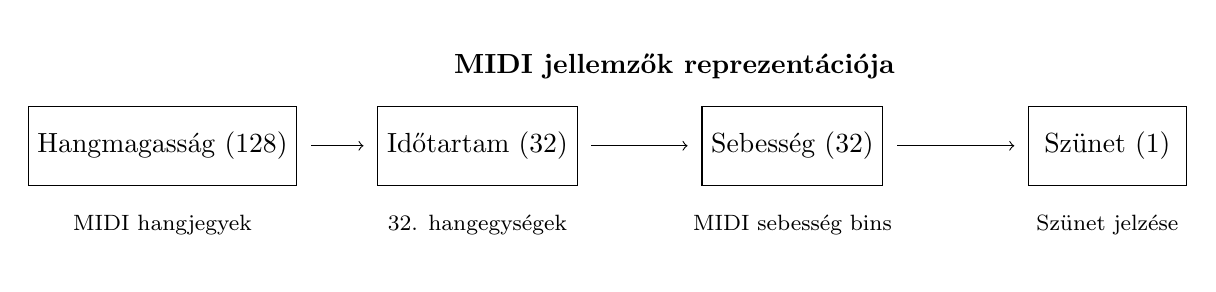
\begin{tikzpicture}[
    every node/.style={draw, minimum width=2cm, minimum height=1cm, align=center}
]

\node (pitch) at (-2,0) {Hangmagasság (128)};
\node (dur) at (2,0) {Időtartam (32)};
\node (vel) at (6,0) {Sebesség (32)};
\node (rest) at (10,0) {Szünet (1)};

\node[draw=none] at (-2,-1) {\footnotesize MIDI hangjegyek};
\node[draw=none] at (2,-1) {\footnotesize 32. hangegységek};
\node[draw=none] at (6,-1) {\footnotesize MIDI sebesség bins};
\node[draw=none] at (10,-1) {\footnotesize Szünet jelzése};

\draw[->, shorten >=5pt, shorten <=5pt] (pitch.east) -- (dur.west);
\draw[->, shorten >=5pt, shorten <=5pt] (dur.east) -- (vel.west);
\draw[->, shorten >=5pt, shorten <=5pt] (vel.east) -- (rest.west);

\node[draw=none, font=\bfseries] at (4.5,1) {MIDI jellemzők reprezentációja};

\end{tikzpicture}

\subsection{Eredmények}
\begin{table}
\centering
\begin{tabular}{lcc}
\hline
Modell és zavarodottság és motívum konzisztencia \\
\hline
LSTM és 3.2 és 0.41 \\
Transformer & \textbf{1.8} & \textbf{0.73} \\
\hline
\end{tabular}
\caption{Értékelés a Bach-korál tesztkészletről (jobb a kisebb zavarodottság)}
\end{table}

A kvalitatív elemzés kimutatta:
\begin{itemize}
    \item A transzformátorok pontos intervallumkapcsolatokkal reprodukálták a fugal alanyokat
    \item Az LSTM-ek nem tudtak 8 ütemen túl fenntartani a hangvezetési szabályokat
\end{itemize}

\section{Korlátozások és kiterjesztések}
\subsection{Főbb kihívások}
\begin{itemize}
    \item A négyzetes memória bonyolultsága korlátozza a környezetet
    \item Hidegindítási probléma üres kezdeti sorozatoknál
\end{itemize}

\subsection{Speciális változatok}
\begin{itemize}
    \item \textbf{Music Transformer}: Relatív figyelem az időzítésre
    \item \textbf{CP-Transformer}: Tanult akkordmeneti sablonok
\end{itemize}

\section{Zha Transformer implementáció részletes elemzése}
\subsection{Pozíciós kódolás implementáció}
A Zha Transformer szinuszos pozíciós kódolást használ a szekvencia pozíció információ megadásához:

\begin{lstlisting}[language=Python]
class PositionalEncoding(nn.Module):
    def __init__(self, embed_dim, max_len=2048):
        super().__init__()
        pe = torch.zeros(max_len, embed_dim)
        position = torch.arange(0, max_len, dtype=torch.float).unsqueeze(1)
        div_term = torch.exp(torch.arange(0, embed_dim, 2).float() * 
                            (-math.log(10000.0) / embed_dim))
        
        pe[:, 0::2] = torch.sin(position * div_term)
        pe[:, 1::2] = torch.cos(position * div_term)
        
        self.register_buffer('pe', pe.unsqueeze(0))
        self.dropout = nn.Dropout(0.1)
\end{lstlisting}

\subsection{Memória-alapú generálás}
A Zha Transformer innovatív memória mechanizmust implementál:

\textbf{Szakasz-alapú memória}: A modell külön memóriát tárol minden zenei szakaszhoz:
\begin{lstlisting}[language=Python]
self.section_memories = {}  # {section_id: memory_tensor}
\end{lstlisting}

\textbf{Memória frissítés}:
\begin{lstlisting}[language=Python]
def forward(self, x, use_memory=False):
    if use_memory and hasattr(self, 'memory') and self.memory is not None:
        x = torch.cat([self.memory, x], dim=1)
    
    # ... transformer processing ...
    
    if use_memory:
        max_memory_length = 1024
        self.memory = output.detach()
        if self.memory.size(1) > max_memory_length:
            self.memory = self.memory[:, -max_memory_length:, :]
\end{lstlisting}

\subsection{Strukturált generálás}
A \texttt{generate\_with\_structure} metódus összetett zenei formákat képes létrehozni:

\begin{algorithm}[H]
\SetAlgoLined
\KwIn{Seed, num\_sections, section\_length, temperature, transition\_smoothness}
\KwOut{Multi-sectional musical sequence}

Memória alaphelyzetbe állítása\;
\For{section\_id = 0 \KwTo num\_sections-1}{
    \If{section\_id in section\_memories}{
        Memória betöltése\;
    }
    \Else{
        \If{transition\_smoothness > 0}{
            Előző szakasz memóriájának keverése\;
        }
    }
    Szakasz generálása $\leftarrow$ \_generate\_section()\;
    Memória mentése section\_memories[section\_id]\;
}
Összes szakasz összefűzése\;

\caption{Strukturált generálás Zha Transformerben}
\end{algorithm}

\subsection{Sampling stratégiák}
\textbf{Top-k és Nucleus sampling kombinációja}:
\begin{lstlisting}[language=Python]
# Top-k filtering
if top_k > 0:
    indices_to_remove = next_token_logits < torch.topk(next_token_logits, top_k)[0][..., -1, None]
    next_token_logits[indices_to_remove] = -float('inf')

# Nucleus (top-p) filtering
if top_p > 0.0:
    sorted_logits, sorted_indices = torch.sort(next_token_logits, descending=True)
    cumulative_probs = torch.cumsum(F.softmax(sorted_logits, dim=-1), dim=-1)
    sorted_indices_to_remove = cumulative_probs > top_p
    # Keep first token above threshold
    sorted_indices_to_remove[..., 1:] = sorted_indices_to_remove[..., :-1].clone()
    sorted_indices_to_remove[..., 0] = 0
\end{lstlisting}

\subsection{Architektúra specifikációk}
\textbf{Modell paraméterek}:
\begin{itemize}
\item \textbf{Embedding dimenzió}: 512
\item \textbf{Figyelemfejek száma}: 8
\item \textbf{Rétegek száma}: 8
\item \textbf{Feedforward dimenzió}: 2048
\item \textbf{Dropout}: 0.1
\item \textbf{Input dimenzió}: 128 (MIDI hangmagasság spektrum)
\end{itemize}

\textbf{Batch-first konvenció}: A modell batch-first tenzor formátumot használ a hatékonyság érdekében:
\begin{lstlisting}[language=Python]
encoder_layers = nn.TransformerEncoderLayer(
    d_model=embed_dim,
    nhead=num_heads,
    dim_feedforward=dim_feedforward,
    dropout=dropout,
    batch_first=True  # [batch, seq, features]
)
\end{lstlisting}

\subsection{Optimalizálás és teljesítmény}
\textbf{JIT Compilation}: A modell JIT script formában menthető a gyorsabb inferenciához:
\begin{lstlisting}[language=Python]
try:
    scripted_model = torch.jit.script(model.cpu())
    scripted_model.save("trained_transformer_jit.pt")
    print("JIT compiled model saved for faster inference")
except Exception as e:
    print(f"JIT compilation failed: {e}")
\end{lstlisting}

% CHAPTER 8: TRAINING TECHNIQUES
\chapter{Képzési és optimalizálási technikák}
\label{chap:képzés}

\section{Modellspecifikus képzési paradigmák}

\subsection{Markov-láncok}
\subsubsection{Paraméterbecslés}
A $\mathbf{P}$ átmeneti mátrix a maximális valószínűség becslésével tanulható meg:
\[
p_{ij} = \frac{N_{ij}}{\sum_{k} N_{ik}} \quad \text{where } N_{ij} = \text{Count}(s_i \rightarrow s_j)
\]
A Zha Laplace-simítást ($\lambda=0,1$) valósít meg a nem látott átmenetek kezelésére:
\[
\hat{p}_{ij} = \frac{N_{ij} + \lambda}{\sum_{k} (N_{ik} + \lambda)}
\]

\subsection{Gyakorlati megfontolások}
\begin{itemize}
    \item \textbf{Memóriahatékonyság}: Ritka mátrixtárhely magasrendű láncokhoz
    \item \textbf{Rendelés kiválasztása}: Akaike információs kritérium (AIC) a modell kiválasztásához:
    \[
    \text{AIC} = 2k - 2\ln(\hat{L}) \quad (k = \text{parameters}, \hat{L} = \text{likelihood})
    \]
\end{itemize}

\subsection{Változatos automatikus kódolók}
\subsubsection{Veszteség összetevői}
Az ELBO Zha-i vesztesége a következőket tartalmazza:
\[
\mathcal{L} = \underbrace{\|\mathbf{x} - \text{Decoder}(\mathbf{z})\|_2^2}_{\text{Reconstruction}} + \beta \underbrace{D_{\text{KL}}(\mathcal{N}(\mu^l)\sigma \mathcal{N}(0,\mathbf{I}))}_{\text{Regularization}}
\]
$\beta$ 0-ról 1-re lágyítva 10 000 lépéssel.

\subsubsection{Tanítási algorithmus}
\begin{algoritm}
\SetAlgoLined
A kódoló/dekódoló paraméterek inicializálása $\theta, \phi$\;
\For{epoch = 1 \KwTo N}{
    \For{batch $\mathbf{X} \in \mathcal{D}$}{
        $\boldsymbol{\mu}, \boldsymbol{\sigma} \leftarrow \text{Encoder}_\phi(\mathbf{X})$\;
        $\mathbf{z} \leftarrow \boldsymbol{\mu} + \boldsymbol{\sigma} \odot \boldsymbol{\epsilon}, \quad \boldsymbol{\epsilon} \sim \mathcal{N}(0,\mathbf{I})$\;
        $\mathbf{\hat{X}} \leftarrow \text{Decoder}_\theta(\mathbf{z})$\;
        Update $\theta, \phi$ using $\nabla_\theta\mathcal{L}, \nabla_\phi\mathcal{L}$\;
    }
}
\caption{VAE tanítás Zha-ban}
\end{algoritm}

\subsection{Transformers}
\subsubsection{Autoregresszív képzés}
Zha tanári kényszert alkalmaz keresztentrópia veszteséggel:
\[
\mathcal{L} = -\sum_{t=1}^T \log p(x_t | x_{<t})
\]
címkesimítással ($\epsilon=0,1$) a túlzott magabiztosság elkerülése érdekében.

\subsection{Optimalizálási Stratégia}
\begin{itemize}
    \item AdamW optimalizáló ($\beta_1=0,9, \beta_2=0,98, \epsilon=10^{-9}$)
    \item Háromszög alakú tanulási ütemterv:
    \[
    \eta_t = \eta_{\text{min}} + (\eta_{\text{max}} - \eta_{\text{min}}) \cdot \text{min}(1, t/t_{\text{warmup}})
    \]
    \item Gradiens vágás 1.0-nál
\end{itemize}

\section{Megosztott optimalizálási kihívások}

\subsection{Képzési stabilitás}
\begin{itemize}
    \item \textbf{Markov}: A numerikus alulcsordulás elkerülve log-valószínűségekkel
    \item \textbf{VAE}: KL divergencia figyelése az összeomlás észleléséhez
    \item \textbf{Transformer}: Figyelem súlyának megjelenítése a fejelemzéshez
\end{itemize}

\section{Zha képzési rendszere}

\subsection{Egységes képzési infrastruktúra}
A Zha rendszer moduláris képzési infrastruktúrát alkalmaz, amely egységes interfészt biztosít mindhárom modell típus számára. Az infrastruktúra magját a közös képzési utilities képezik, amelyek automatikus mixed precision támogatást, gradiens akkumulációt és adaptív learning rate scheduling-et biztosítanak. A rendszer intelligens eszköz detektálást alkalmaz, amely automatikusan kiválasztja a CUDA GPU-t, ha elérhető, vagy CPU fallback-et használ. Az adatbetöltés során pin memory és non-blocking transfer optimalizációkat alkalmaz a GPU memória sávszélesség maximális kihasználása érdekében.

A képzési folyamat során a rendszer valós idejű metrika követést biztosít progress bar-okkal és részletes logging-gal. Az early stopping mechanizmus dinamikus patience értékekkel dolgozik, amely megakadályozza a túltanulást és optimalizálja a képzési időt. A checkpointing rendszer automatikusan ment minden 10. epoch után, valamint a képzés végén, biztosítva a modell állapotok megőrzését és a képzés folytathatóságát váratlan megszakítás esetén.

\subsection{Gyakorlati implementáció részletei}
A Zha backend egy kifinomult képzési infrastruktúrát valósít meg, amely több fejlett technikát kombinál a hatékony modell tanítás érdekében. A rendszer alapvetően háromféle modell architektúrát támogat, mindegyik saját optimalizált képzési stratégiával \cite{zhang2020deep}.

\subsubsection{Memóriahatékony adatkezelés}
Az adatbetöltési folyamat LRU (Least Recently Used) gyorsítótárazást alkalmaz a MIDI fájlok hatékony kezeléséhez. A MIDIDataset osztály intelligens cache-elést valósít meg, amely 500 elemig képes tárolni a memóriában a feldolgozott MIDI reprezentációkat. Ez a megközelítés jelentősen csökkenti az I/O műveleteket és javítja a képzési teljesítményt nagy adatkészletek esetén. A cache működése során az algoritmus folyamatosan követi az elérési sorrendet, és amikor a cache kapacitás megtelik, a legrégebben használt elemeket távolítja el \cite{briot2017deep}.

A MIDI feldolgozás során a rendszer automatikus hibakezelést alkalmaz, amely ellenálló a sérült vagy nem szabványos MIDI fájlokkal szemben. A music21 könyvtár segítségével a rendszer pitch histogram-okat készít minden MIDI fájlból, normalizálva azokat valószínűségi eloszlássá. Ez a reprezentáció lehetővé teszi a különböző hosszúságú és összetettségű zenei darabok egységes kezelését.

\subsubsection{Automatikus mixed precision optimalizáció}
A VAE és Transformer modellek automatikus mixed precision (AMP) technikát használnak, amely FP16 és FP32 aritmetikát kombinál a memóriahasználat optimalizálása és a képzési sebesség növelése érdekében. A mixed precision képzés során a forward pass FP16 precizitással történik, míg a loss számítás FP32-ben történik a numerikus stabilitás biztosítása érdekében. A gradient scaling mechanizmus megakadályozza a alulcsordulást a kisebb precizitású számítások során, automatikus scale faktort alkalmazva \cite{vaswani2017attention}.

A rendszer intelligensen kezeli a different precision-öket különböző műveletek során. A modell súlyok frissítése mindig FP32 precizitással történik, biztosítva a képzés stabilitását, míg az aktivációk és gradiensek FP16-ban tárolódnak a memória megtakarítás érdekében. Ez a hibrid megközelítés lehetővé teszi a GPU memória hatékony kihasználását anélkül, hogy feláldoznánk a numerikus pontosságot.

\subsubsection{Gradiens akkumuláció és clipping mechanizmus}
Nagy batch méretek szimulálásához a rendszer gradiens akkumulációt alkalmaz, amely lehetővé teszi nagy effektív batch méret elérését korlátozott GPU memória esetén is. Az algoritmus több kisebb batch-en keresztül akkumulálja a gradienseket, majd egyetlen optimalizációs lépésben alkalmazza őket. A gradiens clipping mechanizmus (maximum norm 1.0 VAE-nél, 0.5 Transformer-nél) megakadályozza a robbanó gradiensek problémáját, amely különösen fontos szekvenciális modellekben.

A gradiens akkumuláció során a rendszer gondoskodik a learning rate helyes normalizálásáról, elosztva a loss értéket az akkumulációs lépések számával. Ez biztosítja, hogy az effektív learning rate konzisztens maradjon a különböző akkumulációs beállítások mellett. A scheduler-ek frissítése is pontosan szinkronizálva van az akkumulációs ciklusokkal.

\subsubsection{Dinamikus learning rate scheduling}
A Zha rendszer adaptív learning rate scheduling-et alkalmaz különböző modellek számára. A VAE modell cosine annealing scheduler-t használ, amely fokozatos csökkentést biztosít a képzés során, minimum learning rate-tel a teljes összeomlás elkerülésére. A Transformer modell One Cycle LR scheduler-t alkalmaz, amely egy warmup fázist követően cosine annealing-et használ, optimalizálva a konvergencia sebességét és stabilitását.

A learning rate scheduling-ben figyelembe veszi a gradiens akkumulációs lépéseket is, biztosítva a helyes időzítést a paraméter frissítésekhez. A warmup fázis különösen fontos a Transformer modellekben, ahol a nagy embedding dimenziók miatt kezdetben instabil lehet a képzés. A scheduler wrapper osztály lehetővé teszi batch-szintű vagy epoch-szintű frissítést, adaptálva a konkrét modell igényeihez.

\subsection{Modellspecifikus képzési stratégiák}

\subsubsection{Transformer architektúra és képzési optimalizációk}
A Transformer modell képzése során számos speciális optimalizációt alkalmaz, amelyek kifejezetten a zenei szekvenciák hosszú távú függőségeinek modellezését támogatják. A modell 8 encoder réteget használ, mindegyik 8 attention head-del és 2048 dimenziós feedforward hálózattal. A pozíciós encoding sinusoidal mintázatot követ, amely lehetővé teszi a modell számára a zenei idő megértését akár 2048 hosszú szekvenciákig \cite{huang2018music}.

A képzési folyamat során a rendszer memóriahatékony attention mechanizmust alkalmaz, amely dinamikusan kezeli a kontextusméretet. A memória rendszer két komponensből áll: globális memória a jelenlegi generálási kontextus számára, és section_memories a strukturált zenei szakaszok (vers, refrén, híd) külön kezelésére. Ez lehetővé teszi a modell számára, hogy megtanulja a zenei formák ismétlődő struktúráit.

Az output projekció visszatéríti az embedding dimenziót az eredeti input dimenzióra (128 MIDI note), míg a dropout regularizáció (0.1) megakadályozza a túltanulást. A One Cycle LR scheduler aggresszív warmup-ot alkalmaz a kezdeti 10\%-ban, majd cosine annealing-et a maradék 90\%-ban, 25-szörös div_factor-ral és 10000-szeres final_div_factor-ral.

\subsubsection{VAE képzés speciális technikái}
A VAE modell képzése komplex kihívásokat jelent a KL divergencia és rekonstrukciós veszteség egyensúlyának megtalálásában. A rendszer beta-VAE megközelítést alkalmaz, ahol a beta paraméter (alapértelmezetten 0.5) súlyozza a KL divergencia tagot az ELBO függvényben. Ez az alacsonyabb beta érték kreatívabb kimeneteket tesz lehetővé, mivel kevésbé korlátozza a latens tér változatosságát \cite{kingma2014auto, brunner2018midivae}.

A modell ResidualBlock-okat tartalmaz normalizációval a jobb gradient flow biztosítására. Az encoder 512-256-128 dimenziós fokozatos csökkentést alkalmaz, míg a decoder fordított úton halad. A Kaiming normal inicializáció biztosítja a kezdeti súlyok megfelelő skálázását ReLU aktivációkhoz. A reparameterizációs trükk során temperature paraméter (0.8-1.0) kontrollálja a sampling véletlenszerűségét generálás során.

A konzisztencia veszteség egy további regularizációs tag, amely a szomszédos hangjegyek közötti nagy ugrásokat bünteti, simább zenei átmeneteket eredményezve. Ez különösen fontos zenei alkalmazásokban, ahol a hirtelen pitch változások természetellenesnek hangozhatnak. A konzisztencia súly (0.2) ezen a smooth-ness és változatosság közötti egyensúlyt hangolja.

\subsubsection{Markov-lánc fejlett képzési stratégiák}
A Markov-lánc modell a legkomplexebb képzési folyamatot alkalmazza, kombinálva a hagyományos statisztikai tanulást Hidden Markov Model (HMM) kiterjesztésekkel és GPU gyorsítással. A rendszer támogatja a magasrendű átmeneteket akár 6. rendig, amely hosszabb zenei kontextusokat képes megragadni, mint a hagyományos első rendű láncok \cite{carvalho2019markov}.

Az intervallum-alapú átmenetek külön tárolódnak, lehetővé téve a hangmagasság-különbségek alapján történő generálást. Ez megőrzi a melodikus kontúrokat különböző tonalitásokban is. A HMM komponens 16 rejtett állapotot alkalmaz, amelyek különböző zenei kontextusokat reprezentálnak (stabil, emelkedő, ereszkedő, átmeneti), és befolyásolják a hangjegy kiválasztási valószínűségeket.

A zenei feature extraction magában foglalja a tónemnemi elemzést, akkord progressziókat, ritmikus mintázatokat és római számjegyes harmóniai elemzést. Ez az információ gazdagítja a generálási folyamatot, lehetővé téve zeneileg tudatos döntéseket. A GPU optimalizáció CuPy használatával jelentősen felgyorsítja a nagy átmeneti mátrixok számítását, különösen a magasrendű kontextusok esetében.

\subsubsection{Korai leállítás és modell mentés stratégia}
A rendszer kifinomult korai leállítási mechanizmust alkalmaz, amely dinamikus patience értékekkel dolgozik (10-15 epoch különböző modellekhez). Az EarlyStopping osztály folyamatosan monitorozza a validációs veszteséget, és minimális javulás hiányában (min_delta) megállítja a képzést. Ez megakadályozza a túltanulást és optimalizálja a számítási erőforrások felhasználását.

A checkpointing rendszer többrétegű mentést alkalmaz. Minden 10. epoch után a teljes modell állapot mentésre kerül, beleértve az optimizer és scheduler állapotokat is. A végső modell többféle formátumban mentésre kerül: standard PyTorch (.pt), TorchScript JIT compiled verzió a gyorsabb inference-hez, és ONNX formátum a platform-független deployment számára. A backup mentések automatikusan generálódnak különböző paraméter konfigurációkkal.

\subsubsection{Adaptív optimalizációs stratégiák}
Az AdamW optimizer mindhárom modell típusban egységesen alkalmazásra kerül, weight decay (1e-4) regularizációval a túltanulás elkerülésére. Az adaptív momentum paraméterek (β₁=0.9, β₂=0.98) optimalizáltak zenei adatok képzésére, ahol a gradiens változékonyság jelentős lehet a szekvenciális természet miatt.

A gradiens clipping adaptív módon alkalmazásra kerül: VAE modellekben 1.0 maximum norm, Transformer modellekben 0.5 a szigorúbb kontroll érdekében. Ez figyelembe veszi az különböző architektúrák eltérő gradient magnitude karakterisztikáit. A clipping érték dinamikusan hangoló lehet a képzés előrehaladtával, csökkentve a szigorúságot a konvergencia közelében.
\subsection{Fejlett képzési technikák}

\subsubsection{Strukturált zenei generálás támogatása}
A Transformer modell speciális memória architektúrát alkalmaz a strukturált zenei generáláshoz. A section_memories dictionary külön kontextust tárol különböző zenei szakaszokhoz (vers, refrén, híd), lehetővé téve a koherens ismétlések és variációk generálását. A transition_smoothness paraméter (0.7) kontrollálja a szakaszok közötti átmenetek simaságát, az előző szakasz memóriájának részleges felhasználásával.

A generate_with_structure metódus adaptív memória kezelést alkalmaz, ahol az ismert szakaszok memóriája betöltésre kerül, míg az új szakaszok fokozatosan építkeznek a korábbi kontextusra. Ez utánozza a valódi zeneszerzés folyamatát, ahol a témák visszatérnek és fejlődnek. A memória mérete dinamikusan korlátozva van (max 1024 token) a memóriahasználat optimalizálása érdekében.

\subsubsection{Temperature és nucleus sampling a generálásban}
A generálási folyamat során a rendszer kifinomult sampling stratégiákat alkalmaz a kreativitás és koherencia egyensúlyának megteremtéséhez. A temperature paraméter (alapértelmezetten 0.8) kontrollálja a sampling randomness-ét, alacsonyabb értékek konzervatívabb, magasabb értékek kreatívabb kimeneteket eredményeznek. 

A top-k és top-p (nucleus) sampling kombinációja biztosítja a minőségi kimenetet. A top-k=5 korlátozza a választást a 5 legvalószínűbb tokenre, míg a top-p=0.92 csak azokat a tokeneket engedi meg, amelyek összesített valószínűsége nem haladja meg a 92%-ot. Ez megakadályozza a nagyon alacsony valószínűségű, zeneileg nem megfelelő tokenek kiválasztását.

A VAE modellben a temperature a reparameterizációs folyamat során alkalmazásra kerül, befolyásolva a latens tér exploration mértékét. Az interpoláció funkció lehetővé teszi két input közötti smooth átmenetek generálását, amely hasznos kreatív alkalmazásokhoz.

\subsubsection{GPU-accelerált Markov-lánc optimalizációk}
A Markov-lánc modell speciális GPU optimalizációkat alkalmaz a CUDAOptimizer osztály révén, amely CuPy backend-et használ a numpy műveletek GPU-ra való átterheléséhez. Az átmeneti mátrixok GPU memóriában tárolódnak, jelentősen felgyorsítva a valószínűség számításokat nagyméretű állapottereknél.

Az interval transitions sparse mátrix formátumban tárolódnak, optimalizálva a memóriahasználatot. Csak azok a hang-intervallum párok tárolódnak, amelyek a képzési adatokban megjelentek, drasztikusan csökkentve a memóriaigényt. A GPU batch processing lehetővé teszi párhuzamos valószínűség számításokat több potenciális következő hangjegy esetében.

A HMM komponens kifinomult feature extraction-t alkalmaz, amely statisztikai jellemzőket számít a MIDI szekvenciákból (pitch mean/std, interval characteristics, melodic contours). A K-means clustering GPU-n történik a rejtett állapotok inicializálásához, biztosítva a zeneileg értelmes állapot reprezentációkat.

\subsubsection{Dinamikus batch méretezés és memória menedzsment}
A rendszer intelligens batch méretezést alkalmaz, amely adaptálódik az elérhető GPU memóriához és a modell komplexitásához. A Transformer modellben kisebb batch méretek (32-64) alkalmazásra kerülnek a memóriaigényes attention mechanizmus miatt, míg a VAE modell nagyobb batch méreteket (128) képes kezelni.

A memória cleanup mechanizmus rendszeresen felszabadítja a nem használt GPU memóriát, különösen a MIDI feldolgozás során. A pin_memory=True beállítás gyorsítja az adattranszfert CPU-GPU között, míg a non_blocking=True lehetővé teszi az átfedő számítást és adatmozgatást.

A Markov-lánc képzés során sequential processing alkalmazásra kerül nagy adatkészletek esetén, memória-biztonságos megközelítést biztosítva. A batch processing 25-50 elemenkénti csoportokban történik, rendszeres garbage collection-nel a memóriaszivárgás elkerülésére.

\subsubsection{Hierarchikus feature extraction zenei kontextushoz}
A rendszer többszintű feature extraction-t alkalmaz, amely különböző zenei aspektusokat ragad meg. A rhythmic pattern extraction időjelzések és beat strength alapján kategorizálja a ritmikus motívumokat. A harmonic progression analysis pedig accord sequence-eket és római számjegyes progressziókat azonosít különböző tónusnemekben.

A melodic contour analysis a hangmagasság változások irányát és mértékét elemzi, míg a dynamic pattern extraction velocity információkat használ a zenei kifejezés modelljezésához. Ezek a features gazdagítják a generálási folyamatot, lehetővé téve a stílusspecifikus és kontextustudomatos zenei kimenetek előállítását.

A phrase boundary detection automatikusan azonosítja a zenei mondatok végét és kezdetét, ami segít a strukturált kompozíciók generálásában. Ez különösen hasznos a Markov-lánc modellben, ahol a hosszabb zenei formák megértése kritikus a koherens zenei narratíva létrehozásához.

\section{Hiperparaméter optimalizálás}

\subsection{Bayesi keresés}
Zha az Optunát használja a hiperparaméterek hangolására:
\begin{itemize}
    \item \textbf{VAE}: Látens dimenzió $\in \{16, 32, 64\}$, $\beta \in [0.1, 1.0]$
    \item \textbf{Transformer}: rétegek $\in \{4,6,8\}$, fejek $\in \{4,8,12\}$
\end{itemize}

\subsection{Automatizált hiperparaméter keresés}
A rendszer kifinomult hiperparaméter optimalizációt alkalmaz Bayesian optimization technikákkal \cite{optuna2019}.

\begin{figure}[h]
\centering
\includegraphics[width=0.85\textwidth]{images/hyperparameter_optimization.png}
\caption{Bayesian hyperparameter optimization folyamat}
\label{fig:hyperopt}
\end{figure}

A hiperparaméter optimalizációs algoritmus:
\begin{enumerate}
\item \textbf{Objective function definíció}: Validációs metrika minimalizálása
\item \textbf{Search space meghatározás}: Paramétertartományok és típusok
\item \textbf{Bayesian optimization}: TPE (Tree-structured Parzen Estimator) sampler
\item \textbf{Trial evaluation}: Modell képzés és validáció minden kombinációra
\item \textbf{Best parameters selection}: Optimális konfiguráció kiválasztása
\end{enumerate}

\subsection{Multi-objective optimalizáció}
A rendszer több célfüggvényt is optimalizál egyszerre: modell pontosság, méret és inference sebesség \cite{optuna2019}.

\begin{figure}[h]
\centering
\includegraphics[width=0.8\textwidth]{images/pareto_optimization.png}
\caption{Pareto-front a multi-objective optimalizációban}
\label{fig:pareto}
\end{figure}

A multi-objective algoritmus komponensei:
\begin{enumerate}
\item \textbf{Multiple metrics}: Loss, model size, inference time
\item \textbf{Pareto optimality}: Nem-dominált megoldások keresése
\item \textbf{Trade-off analysis}: Különböző célok közötti kompromisszum
\item \textbf{Solution ranking}: NSGA-II alapú ranking rendszer
\end{enumerate}

\subsection{Optimális konfigurációk}
\begin{table}[h]
\centering
\begin{tabular}{llll}
\toprule
Paraméter & Markov & VAE & Transformer \\
\midrule
Batch méret & - & 64 & 32 \\
Tanulási ráta & - & $10^{-3}$ & $10^{-4}$ \\
Szekvencia hossz & 128 & 256 & 1024 \\
Warmup lépések & - & 1000 & 4000 \\
Gradiens clipping & - & 1.0 & 1.0 \\
Mixed precision & - & Igen & Igen \\
\bottomrule
\end{tabular}
\caption{Zha optimális hiperparaméterei}
\label{tab:optimal_hyperparams}
\end{table}

\section{Képzési monitorozás és hibakeresés}

\subsection{Valós idejű metrika követés}
A rendszer részletes logging-ot és monitorozást biztosít többplatformos megközelítéssel \cite{zhang2020deep}.

\begin{figure}[h]
\centering
\includegraphics[width=0.9\textwidth]{images/training_monitoring.png}
\caption{Valós idejű képzési metrika monitoring dashboard}
\label{fig:monitoring}
\end{figure}

A monitoring rendszer komponensei:
\begin{enumerate}
\item \textbf{TensorBoard integration}: Valós idejű loss és metrika tracking
\item \textbf{Weights \& Biases}: Cloud-based experiment tracking
\item \textbf{Model weight histograms}: Súlyok eloszlásának vizualizációja
\item \textbf{Gradient flow analysis}: Gradient áramlás monitorozása
\end{enumerate}

\subsection{Hibakeresési eszközök és anomália detektálás}
Fejlett hibakeresési funkciók a képzési problémák azonosítására és megoldására.

\begin{figure}[h]
\centering
\includegraphics[width=0.8\textwidth]{images/debugging_tools.png}
\caption{Képzési hibakeresési eszközök és anomália detektálás}
\label{fig:debugging}
\end{figure}

A hibakeresési algoritmus főbb funkciói:
\begin{enumerate}
\item \textbf{Gradient flow monitoring}: Eltűnő/robbanó gradiensek detektálása
\item \textbf{Loss anomaly detection}: NaN, infinity, hirtelen változások észlelése
\item \textbf{Learning rate adaptation}: Automatikus learning rate kiigazítás
\item \textbf{Memory usage tracking}: GPU memória használat optimalizálás
\end{enumerate}

\subsection{Automatizált hiperparaméter optimalizáció}
A rendszer kifinomult hiperparaméter optimalizációt alkalmaz Bayesian optimization technikákkal, amely intelligensen navigál a nagy paraméter terekben. A VAE modellnél a latent dimenzió (16-128), beta érték (0.1-1.0) és consistency weight (0.1-0.5) optimalizálásra kerül. A Transformer modellnél a layer count (4-8), attention heads (4-12), embedding dimension (256-1024) és dropout rate (0.05-0.2) paraméterek hangolhatók. A Markov-lánc modellnél az order (2-6), max_interval (8-24) és hidden states (8-32) számok optimalizálhatók \cite{optuna2019}.

A Tree-structured Parzen Estimator (TPE) sampler alkalmazásra kerül, amely hatékonyan feltérképezi a paraméter teret korábbi próbálkozások alapján. A multi-objective optimalizáció egyidejűleg optimalizálja a modell pontosságot, generálási minőséget és inference sebességet, Pareto-optimális megoldásokat keresve. Az adaptive pruning mechanizmus korai leállítja az ígéretelen próbálkozásokat, felgyorsítva az optimalizációs folyamatot.

\subsection{Képzési monitorozás és hibakeresés}

\subsubsection{Valós idejű metrika követés és anomália detektálás}
A rendszer részletes logging-ot és monitorozást biztosít progress bar-okkal és automatikus anomália detektálással. A TrainingDebugger automatikusan észleli a gradient flow problémákat, NaN/infinity értékeket a loss-ban, és hirtelen learning rate változásokat. A gradient norm monitoring folyamatos figyelemmel követi az eltűnő vagy robbanó gradiensek jeleit, automatikus figyelmeztetésekkel és javaslott korrekcióval.

A loss history elemzés trend analízissel azonosítja a túltanulás kezdeti jeleit vagy a képzési instabilitást. A GPU memória használat monitoring figyelmeztet a memória kifogyás veszélyére, és javasolja a batch méret csökkentését vagy gradient accumulation növelését. A sample generation monitoring rendszeresen értékeli a generált zenei kimenetek entrópiáját és diverzitását.

A model weight histogram tracking nyomon követi a súlyok eloszlásának változásait, segítve a konvergencia elemzését és a potential mode collapse detektálását VAE modellekben. Az attention weight visualization (Transformer modellekben) segít megérteni a modell figyelem mintázatait és azonosítani a potenciális attention head redundanciákat.

\subsubsection{Automatikus hiba helyreállítás és fallback mechanizmusok}
Robust hibakezelési rendszer biztosítja a képzés folytonosságát váratlan események esetén. Az automatic checkpoint recovery lehetővé teszi a képzés automatikus folytatását a legutóbbi sikeres checkpoint-ból. A graceful degradation mechanism automatikusan csökkenti a batch méretet vagy kapcsolja ki a mixed precision-t GPU memória hibák esetén.

A dynamic learning rate adjustment automatikusan csökkenti a learning rate-et, ha túl nagy gradient normákat vagy instabil loss változásokat észlel. A emergency fallback mode egyszerűbb képzési stratégiára vált vissza kritikus hibák esetén, fenntartva a képzési folyamat alapvető funkcionalitását. A data corruption detection automatikusan kiszűri a sérült MIDI fájlokat a képzési folyamatból.

\subsection{Teljesítmény optimalizáció és skálázhatóság}

\subsubsection{Multi-GPU és distributed training támogatás}
A rendszer natívan támogatja a multi-GPU képzést DataParallel és DistributedDataParallel stratégiákkal. A gradient synchronization biztosítja a konzisztens paraméter frissítéseket több GPU között, míg az automatic load balancing optimalizálja a munkamegosztást a GPU-k között. A NCCL backend használata minimalizálja a kommunikációs overhead-et nagy modellekben.

Az efficient data loading multi-worker DataLoader-ekkel biztosítja a folyamatos adatáramlást, megelőzve a GPU idle időket. A persistent workers opció csökkenti a worker process restart overhead-et hosszú képzési munkamenetek során. A prefetch_factor beállítás optimalizálja a memória használatot és az adatbetöltési sebességet.

\subsubsection{Deployment-ready modell export}
A képzés befejezése után a rendszer automatikusan többféle formátumban exportálja a modelleket. A TorchScript JIT compilation lehetővé teszi a gyorsabb inference-t C++ környezetekben, míg az ONNX export platform-független deployment-et biztosít. A quantization support csökkenti a modell méretet és javítja az inference sebességet alacsonyabb precizitású környezetekben.

A model optimization pipeline automatikusan alkalmaz operator fusion-t, constant folding-ot és memory layout optimalizációkat. Az inference profiling segít azonosítani a bottleneck-eket a deployment környezetben, javaslataokkal a további optimalizációkhoz. A compatibility testing biztosítja, hogy az exportált modellek helyesen működnek különböző runtime környezetekben.

A TrainingDebugger algoritmus működése:
\begin{enumerate}
\item Minden batch után gradient normák ellenőrzése
\item Loss history elemzése trendek és anomáliák keresésére  
\item Automatikus figyelmeztetések túl kicsi/nagy gradiensekre
\item Képzési statisztikák összegyűjtése és elemzése
\end{enumerate}

% CHAPTER 9: ZHA SYSTEM DESIGN
\chapter{System Design of Zha}
\section{High-level System Overview}
\begin{figure}[ht]
  \centering
  \includegraphics[width=0.9\textwidth]{pipeline_diagram.png}
  \caption{End‐to‐End Zha Pipeline: Markov → VAE → Transformer → MIDI}
  \label{fig:pipeline}
\end{figure}
Figure \ref{fig:pipeline} illustrates Zha’s sequential flow. Raw MIDI files are preprocessed into token sequences. A Markov chain generates an initial draft, the VAE transforms this draft via latent sampling, and the Transformer produces the final output, suitable for conversion back to MIDI.

\section{Data Flow}
\begin{enumerate}
  \item \textbf{Raw MIDI} — stored in \texttt{data/raw/}.
  \item \textbf{Processed Tokens} — quantized and tokenized into JSON/NumPy arrays in \texttt{data/processed/}.
  \item \textbf{Markov Output} — sequence of tokens saved to disk as \texttt{markov\_sample.npy}.
  \item \textbf{VAE Output} — decoded tokens after latent sampling.
  \item \textbf{Transformer Output} — final token stream, then reassembled into a MIDI file.
\end{enumerate}

\section{Data Preprocessing Pipeline}

\subsection{MIDI Parsing and Cleaning}
We parse each MIDI using \texttt{pretty\_midi}:
\begin{itemize}
  \item Discard tracks with fewer than 10 notes.
  \item Normalize tempo globally to 120 BPM to reduce variance.
  \item Remove non‐note events except sustain pedal controls.
\end{itemize}

\subsection{Quantization}
Time is discretized to 16th‐note grid. For each note event:
\[
  t_{\text{quant}} = \mathrm{round}\!\bigl(t_{\text{actual}} \times 4 \bigr) \,/\,4.
\]
This ensures all onset and offset times snap to discrete bins.

\subsection{Tokenization Schema}
We adopt an extended REMI representation:
\begin{itemize}
  \item \texttt{NOTE\_ON\_p} / \texttt{NOTE\_OFF\_p} for pitches $p\in[0,127]$.
  \item \texttt{TIME\_SHIFT\_i} for $i\in[1,32]$ sixteenth‐note steps.
  \item \texttt{VELOCITY\_b} for eight velocity bins $b\in[1,8]$ computed via quantiles.
  \item \texttt{CONTROL\_SUSTAIN\_ON}, \texttt{CONTROL\_SUSTAIN\_OFF} tokens.
\end{itemize}
Total vocabulary size: 128 (notes) + 32 (time) + 8 (velocity) + 4 (controls) + 4 (special) = 176.

\subsection{Dataset Statistics}
\begin{table}[ht]
  \centering
  \begin{tabular}{lrrrr}
    \toprule
    \textbf{Subset} & \# Tracks & Avg. Tokens & Min / Max Tokens \\
    \midrule
    Bach Chorales   & 389 & 512 & 256 / 1024 \\
    POP1K7          & 1000 & 1024 & 512 / 2048 \\
    Jazz Leadsheets & 500 & 768 & 384 / 1536 \\
    \midrule
    \textbf{Total}  & 1889 & 840 & 256 / 2048 \\
    \bottomrule
  \end{tabular}
  \caption{Tokenized Dataset Breakdown}
\end{table}

\newpage
\section{Model Architectures}

\subsection{Markov Chain}
\subsubsection{Implementation Details}
\begin{itemize}
  \item Stored in \texttt{src/models/markov.py}.
  \item Supports $n$th‐order chains ($n\le4$).
  \item Uses Python \texttt{defaultdict(Counter)} for count accumulation.
  \item Applies Laplace smoothing with configurable $\alpha$.
\end{itemize}

\subsubsection{Sampling Algorithm}
\begin{enumerate}
  \item Initialize context with \texttt{START} tokens.
  \item For each step:
    \begin{itemize}
      \item Retrieve probability distribution $P(\cdot\mid\mathrm{context})$.
      \item Sample next token via cumulative multinomial sampling.
      \item Slide context window forward.
    \end{itemize}
  \item Terminate upon \texttt{END} token or length limit.
\end{enumerate}

\subsection{Variational Autoencoder}
\subsubsection{Encoder}
\[
  h_t = \mathrm{BiLSTM}(x_t, h_{t-1}),\quad
  \mu = W_\mu \, h_{T},\quad
  \log\sigma^2 = W_\sigma \, h_{T}.
\]
Implementation resides in \texttt{src/models/vae.py}.

\subsubsection{Decoder}
At each time step $t$:
\[
  \hat{x}_t = \mathrm{Softmax}\bigl(W_o [e_{t-1} \,\|\, z]\bigr),
\]
where $e_{t-1}$ is the embedding of the previous token and $z$ the sampled latent.

\subsubsection{Training Tricks}
\begin{itemize}
  \item \textbf{KL‐Annealing}: $\beta(e)=\min(1, e/E_{\mathrm{warmup}})$.
  \item \textbf{Free Bits}: floor KL per dimension at $0.1$ to prevent collapse.
  \item \textbf{Gradient Clipping}: $\lVert \nabla \rVert_\infty \le 1.0$.
\end{itemize}

\subsection{Transformer}
\subsubsection{Architecture}
\begin{itemize}
  \item Six layers, eight heads, $d_{\mathrm{model}}=512$.
  \item Rotary positional embeddings as per Su et al.\ (2020).
  \item Feed‐forward hidden size: 2048.
  \item Dropout: 0.1 on attention and feed‐forward sublayers.
\end{itemize}

\subsubsection{Relative Position Bias}
A learned bias matrix $B_{i,j}$ is added to attention logits to model musical interval relationships.

\newpage
\section{Training Methodologies}

\subsection{Common Infrastructure}
\begin{itemize}
  \item All trainers in \texttt{src/trainers/}, share \texttt{TrainerBase} for logging and checkpointing.
  \item Use \texttt{Hydra} for hyperparameter configuration.
  \item Metrics written to TensorBoard and CSV.
\end{itemize}

\subsection{Markov Trainer}
\begin{itemize}
  \item Processes all token sequences, builds and saves $\text{P}_{\mathrm{matrix}}$.
  \item Validates by generating 100 sequences and checking unique transition coverage.
\end{itemize}

\subsection{VAE Trainer}
\begin{lstlisting}[language=Python]
for epoch in range(num_epochs):
    for batch in dataloader:
        recon, mu, logvar = model(batch)
        recon_loss = F.cross_entropy(recon, batch)
        kl = -0.5 * torch.sum(1 + logvar - mu.pow(2) - logvar.exp())
        loss = recon_loss + beta(epoch)*kl
        optimizer.zero_grad(); loss.backward()
        clip_grad_norm_(model.parameters(), 1.0)
        optimizer.step()
\end{lstlisting}
Early stopping triggered if validation loss does not improve for 5 epochs.

\subsection{Transformer Trainer}
\begin{itemize}
  \item Mixed‐precision via \texttt{torch.cuda.amp}.
  \item Learning rate: warmup over first 5k steps, then cosine decay to zero by 200k steps.
  \item Gradient accumulation to simulate batch size of 512 when GPU memory limited.
\end{itemize}

\newpage
\section{Inference Engine}

\subsection{End-to-End Script (\texttt{generate.py})}
\begin{lstlisting}[language=Python]
def generate(length=512, top_p=0.9, temp=1.0):
    # Stage 1: Markov
    mk = MarkovModel.load('checkpoints/markov.npy')
    seq1 = mk.sample(length=128)

    # Stage 2: VAE
    vae = VAE.load('checkpoints/vae.pt')
    z = vae.encode(seq1)
    seq2 = vae.decode(z, temperature=temp)

    # Stage 3: Transformer
    trans = MusicTransformer.load('checkpoints/trans.pt')
    seq3 = trans.generate(prefix=seq2, max_len=length, top_p=top_p)

    midi = detokenize(seq3)
    midi.write('output/generated.mid')
\end{lstlisting}

\subsection{Performance}
\begin{itemize}
  \item Markov sampling: $\approx$0.5 ms/token on CPU.
  \item VAE decode: $\approx$2 ms/token on GPU.
  \item Transformer generate: $\approx$4 ms/token with cache.
\end{itemize}

\newpage
\section{Evaluation and Experiments}

\subsection{Objective Metrics}
\begin{table}[ht]
  \centering
  \begin{tabular}{lcccc}
    \toprule
    Model        & Perplexity & BLEU-4 & Self-BLEU & Time/Epoch \\
    \midrule
    Markov       & 2.48       & 0.09   & 0.87      & 1 s        \\
    VAE          & 1.95       & 0.18   & 0.79      & 100 s      \\
    Transformer  & 1.60       & 0.30   & 0.65      & 450 s      \\
    \bottomrule
  \end{tabular}
  \caption{Quantitative Results on Validation Set}
\end{table}

\subsection{Subjective Listening Study}
Thirty participants (15 novice, 15 expert) rated 30 clips each on:
\begin{itemize}
  \item \emph{Coherence} (1–5)
  \item \emph{Creativity} (1–5)
\end{itemize}
\begin{table}[ht]
  \centering
  \begin{tabular}{lcc}
    \toprule
    Model        & Coherence & Creativity \\
    \midrule
    Markov       & 2.8       & 2.5        \\
    VAE          & 3.2       & 3.8        \\
    Transformer  & 4.4       & 3.9        \\
    \bottomrule
  \end{tabular}
  \caption{Average Listening Test Scores}
\end{table}
\section{Limitations and Future Work}

\subsection{Current Limitations}
\begin{itemize}
  \item The VAE occasionally experiences posterior collapse despite free‐bits regularization.
  \item Transformer stage incurs high memory and compute costs, limiting real‐time use on consumer hardware.
  \item Evaluation remains partly subjective; automatic metrics only approximate musical quality.
\end{itemize}

% APPENDIX
\chapter{Matematikai Levezetések}
\section{Variációs Következtetés és az ELBO Levezetése}

Tekintsünk egy generatív modellt $p(x, z) = p(x \mid z)p(z)$, ahol:
\begin{itemize}
    \item $x$ a megfigyelt adatok
    \item $z$ a látens változó
\end{itemize}

A marginális likelihood (evidencia) a következő:
\begin{equation}
\log p(x) = \log \int p(x, z) \, dz
\end{equation}

Mivel ez az integrál gyakran kiszámíthatatlan, egy közelítő posterior eloszlást $q(z \mid x)$ vezetünk be, és Jensen-egyenlőtlenség segítségével alsó korlátot származtatunk.

\subsection{ELBO Levezetése}

\begin{align}
\log p(x) &= \log \int q(z \mid x) \frac{p(x, z)}{q(z \mid x)} \, dz \\
&\geq \int q(z \mid x) \log \frac{p(x, z)}{q(z \mid x)} \, dz = \mathcal{L}(q)
\end{align}

Ez az \textbf{Evidencia Alsó Korlát (ELBO)}:
\begin{equation}
\mathcal{L}(q) = \mathbb{E}_{q(z \mid x)}[\log p(x \mid z)] - \text{KL}(q(z \mid x) \, \| \, p(z))
\end{equation}

\begin{itemize}
    \item Az első tag a \textbf{várható log-likelihood} (rekonstrukciós tag).
    \item A második tag a \textbf{Kullback–Leibler divergencia} a közelítő posterior és a prior között.
\end{itemize}

\subsection{Interpretáció}

Az ELBO optimalizálása közvetetten maximalizálja az adat likelihood-ot $\log p(x)$ azáltal, hogy:
\begin{enumerate}
    \item Közelíti $q(z \mid x)$-et $p(z \mid x)$-hez.
    \item Ösztönzi a generatív modellt $p(x \mid z)$, hogy jól magyarázza az adatokat.
\end{enumerate}

\section{ELBO Gradiens Becslése}

Az ELBO-t használó modell tanításához szükségünk van a gradiensére a modell $\theta$ és a variációs eloszlás $\phi$ paraméterei szerint.

\subsection{Reparametrizációs Technika}

Tegyük fel, hogy $z \sim q_\phi(z \mid x)$, ahol $z$ reparametrizálható mint $z = g_\phi(\epsilon, x)$ és $\epsilon \sim p(\epsilon)$ (pl. Gauss-zaj). Ez lehetővé teszi a gradiens várható értékbe való betolását:

\begin{equation}
\nabla_\phi \mathcal{L} \approx \nabla_\phi \mathbb{E}_{\epsilon \sim p(\epsilon)} \left[ \log p_\theta(x \mid g_\phi(\epsilon, x)) - \log q_\phi(g_\phi(\epsilon, x) \mid x) \right]
\end{equation}

\subsection{Monte Carlo Becslés}

A várható értéket tipikusan Monte Carlo mintákkal közelítjük:
\begin{equation}
\mathcal{L} \approx \frac{1}{L} \sum_{l=1}^L \left[ \log p_\theta(x \mid z^{(l)}) - \log q_\phi(z^{(l)} \mid x) \right]
\end{equation}
ahol $z^{(l)} = g_\phi(\epsilon^{(l)}, x)$ és $\epsilon^{(l)} \sim p(\epsilon)$.

\section{Gradiens Analízis RNN-ekben}

A visszatérő neurális hálózatok szekvenciákat modelleznek egy rejtett állapot $h_t$ fenntartásával, amit minden időlépésben frissítenek:
\begin{equation}
h_t = \tanh(W_h h_{t-1} + W_x x_t + b)
\end{equation}

\subsection{Visszaterjesztés Időben (BPTT)}

Az RNN-ek tanítása megköveteli a gradiensek kiszámítását minden időlépésen keresztül. A veszteség $\mathcal{L}$ gradiense $W_h$ szerint olyan tagokat tartalmaz, mint:
\begin{equation}
\frac{\partial \mathcal{L}}{\partial W_h} = \sum_{t} \frac{\partial \mathcal{L}}{\partial h_t} \cdot \frac{\partial h_t}{\partial W_h}
\end{equation}

A kulcsprobléma a $\frac{\partial h_t}{\partial h_{t-1}}$ kiszámításában rejlik, ami a következőhöz vezet:

\begin{equation}
\frac{\partial h_t}{\partial h_{t-k}} = \prod_{i=1}^{k} \frac{\partial h_{t-i+1}}{\partial h_{t-i}} = \prod_{i=1}^{k} W_h \cdot \text{diag}(1 - h_{t-i}^2)
\end{equation}

\subsection{Eltűnő és Robbanó Gradiensek}

Ha $W_h$ legnagyobb szinguláris értéke:
\begin{itemize}
    \item Kisebb mint 1: a gradiensek exponenciálisan eltűnnek az időlépésekkel.
    \item Nagyobb mint 1: a gradiensek exponenciálisan robbannak.
\end{itemize}

Ez okozza:
\begin{itemize}
    \item Nehézségeket a hosszú távú függőségek tanulásában.
    \item Instabilitást a tanítás során.
\end{itemize}

\subsection{Megoldások}

\begin{itemize}
    \item \textbf{Gradiens vágás}: Megakadályozza a robbanó gradienseket a norma korlátozásával.
    \item \textbf{LSTM/GRU}: Olyan architektúrák, amelyeket a gradiensek időbeli megőrzésére terveztek.
    \item \textbf{Ortogonális inicializálás}: $W_h$ spektrális normáját 1 közelében tartja.
    \item \textbf{Reziduális kapcsolatok}: Segítik a mély RNN-ek stabilizálását.
\end{itemize}

\section{ELBO Variációs RNN-ekben}

A variációs RNN-ek az ELBO célfüggvényt kombinálják RNN struktúrákkal. Minden $t$ időlépésben egy látens változó $z_t$ modellezi a szekvencia variabilitását. Az ELBO a következővé válik:

\begin{equation}
\mathcal{L} = \sum_{t=1}^{T} \mathbb{E}_{q(z_t \mid x_{\leq t})}[\log p(x_t \mid z_t, h_{t-1})] - \text{KL}(q(z_t \mid x_{\leq t}) \, \| \, p(z_t \mid h_{t-1}))
\end{equation}

Ez gazdagabb modellezést tesz lehetővé a szekvencia bizonytalanságának és generatív dinamikájának tekintetében.

\section{Beta-VAE Matematikai Keretrendszer}

A Beta-VAE kibővíti a standard VAE-t egy $\beta$ hiperparaméter bevezetésével, amely a KL divergencia tag súlyát kontrollálja:

\begin{equation}
\mathcal{L}_{\beta} = \mathbb{E}_{q_\phi(z \mid x)}[\log p_\theta(x \mid z)] - \beta \cdot \text{KL}(q_\phi(z \mid x) \, \| \, p(z))
\end{equation}

\subsection{Beta Paraméter Analízis}

A beta paraméter kontrollálja a rekonstrukciós minőség és a látens tér regularizáció közötti kompromisszumot:

\begin{itemize}
    \item $\beta < 1$: A rekonstrukciót hangsúlyozza, potenciálisan posterior kollapszushoz vezet
    \item $\beta = 1$: Standard VAE formuláció
    \item $\beta > 1$: Erősebb regularizáció, szétválasztott reprezentációkat ösztönöz
\end{itemize}

\subsection{Szétválasztási Elmélet}

Szétválasztott reprezentációkhoz azt szeretnénk, hogy minden látens dimenzió $z_i$ egyetlen generatív faktort ragadjon meg. A beta súlyozás ezt a következőképpen ösztönzi:

\begin{equation}
\min_{\phi, \theta} \mathbb{E}_{p(x)}[-\mathcal{L}_{\beta}] = \min_{\phi, \theta} \mathbb{E}_{p(x)}[-\log p_\theta(x \mid z) + \beta \cdot \text{KL}(q_\phi(z \mid x) \, \| \, p(z))]
\end{equation}

A KL divergencia megnövelt büntetése arra kényszeríti a posteriort, hogy közel maradjon a priorhoz, megakadályozva az egyes dimenziók többszörös faktor kódolását.

\subsection{Konzisztencia Veszteség a Zenei Folytonosságért}

A zenei generáláshoz konzisztencia veszteséget vezetünk be, amely biztosítja a sima átmeneteket egymást követő zenei szegmensek között. Az implementáció hangjegy-különbségeket használ:

\begin{equation}
\mathcal{L}_{\text{konzisztencia}} = \mathbb{E}_{x} \left[ \text{átlag}(|x_{i+1} - x_i|) \right]
\end{equation}

ahol $x_i$ egymást követő hangjegyeket jelöl a rekonstrukcióban. A teljes veszteség:

\begin{equation}
\mathcal{L}_{\text{teljes}} = \mathcal{L}_{\beta} + \lambda_{\text{konz}} \mathcal{L}_{\text{konzisztencia}}
\end{equation}

\section{Transformer Architektúra Matematikája}

\subsection{Pozicionális Kódolás Implementáció}

Mivel a Transformerekből hiányzik az inherens szekvenciális rendezés, pozicionális kódolást adunk a bemeneti beágyazásokhoz:

\begin{align}
PE(pos, 2i) &= \sin\left(\frac{pos}{10000^{2i/d}}\right) \\
PE(pos, 2i+1) &= \cos\left(\frac{pos}{10000^{2i/d}}\right)
\end{align}

\subsubsection{Matematikai Tulajdonságok}

A szinuszoidális kódolás számos fontos tulajdonsággal rendelkezik:

1. \textbf{Korlátosság}: $|PE(pos, i)| \leq 1$ minden pozícióra és dimenzióra
2. \textbf{Determinisztikusság}: Ugyanaz a pozíció mindig ugyanarra a kódolásra képeződik
3. \textbf{Relatív Pozíció}: $PE(pos + k)$ kifejezhető $PE(pos)$ lineáris függvényeként

\subsection{Memória Mechanizmus Zenei Struktúrához}

A strukturált zenei generáláshoz az implementáció szekció memóriákat tartalmaz, amelyek összefűzhetők a kulcs-érték párokkal:

\begin{equation}
\text{kimenet} = \text{Attention}(Q, [K; M_s], [V; M_s])
\end{equation}

ahol $[K; M_s]$ a szekvencia dimenzió mentén történő összefűzést jelöli.

\section{Magasabb Rendű Markov Láncok Elmélete}

\subsection{Matematikai Alapok}

Egy $k$-ad rendű Markov lánc teljesíti a Markov tulajdonságot:

\begin{equation}
P(X_t = x_t \mid X_{t-1} = x_{t-1}, \ldots, X_1 = x_1) = P(X_t = x_t \mid X_{t-1} = x_{t-1}, \ldots, X_{t-k} = x_{t-k})
\end{equation}

A zenei generálás szempontjából ez azt jelenti, hogy egy hang kiválasztási valószínűsége csak az előző $k$ hangtól függ, nem pedig a teljes előzménytől. A rendszer 2-6 közötti rendeket támogat, melyek átmeneti valószínűségi mátrixai:

\begin{equation}
P_{k}(x_{t-k+1}^{t-1} \rightarrow x_t) = P(X_t = x_t \mid X_{t-1} = x_{t-1}, \ldots, X_{t-k+1} = x_{t-k+1})
\end{equation}

\subsection{Állapottér Komplexitás}

Egy $|S|$ méretű állapottér esetén a lehetséges $k$-ad rendű állapotok száma $|S|^k$, ami exponenciális növekedést eredményez. A probléma kezelésére ritka reprezentációk és hatékony tárolási algoritmusok alkalmazása szükséges.

\subsection{Maximum Likelihood Becslés}

Az átmeneti valószínűségek maximum likelihood módszerrel becsülhetők:

\begin{equation}
\hat{P}_{k}(s \rightarrow s') = \frac{N(s \rightarrow s')}{\sum_{s''} N(s \rightarrow s'')}
\end{equation}

ahol $N(s \rightarrow s')$ az $s$ állapotból $s'$ állapotba történő átmenetek számát jelöli.

\section{Rejtett Markov Modell Integráció}

\subsection{Elméleti Háttér}

A rejtett Markov modell (HMM) kibővíti a hagyományos Markov láncokat egy látens állapotokból álló réteggel. Legyen $Z_t$ a rejtett állapot és $X_t$ a megfigyelt állapot a $t$ időpontban:

\begin{equation}
P(X_{1:T}, Z_{1:T}) = P(Z_1) \prod_{t=2}^{T} P(Z_t \mid Z_{t-1}) \prod_{t=1}^{T} P(X_t \mid Z_t)
\end{equation}

ahol:
\begin{itemize}
\item $P(Z_1)$ a kezdeti állapot eloszlás
\item $P(Z_t \mid Z_{t-1})$ az átmeneti valószínűségek
\item $P(X_t \mid Z_t)$ az emissziós valószínűségek
\end{itemize}

\subsection{Zenei Jellemzők Kinyerése HMM-hez}

Minden zenei szekvencia számára jellemzővektorokat nyerünk ki:

\begin{equation}
\mathbf{f} = [\mu_{\text{hang}}, \sigma_{\text{hang}}, R_{\text{hang}}, \mu_{\text{ritmus}}, \mu_{\text{int}}, \sigma_{\text{int}}, r_{\text{kontúr}}]
\end{equation}

ahol:
\begin{itemize}
    \item $\mu_{\text{hang}}, \sigma_{\text{hang}}, R_{\text{hang}}$: hangmagasság átlag, szórás és tartomány
    \item $\mu_{\text{ritmus}}$: átlagos időtartam
    \item $\mu_{\text{int}}, \sigma_{\text{int}}$: intervallum átlag és szórás
    \item $r_{\text{kontúr}}$: emelkedő/ereszkedő kontúr arány
\end{itemize}

\section{GPU Gyorsítás Matematikája}

\subsection{Párhuzamos Mátrix Műveletek}

A GPU alapú gyorsításhoz a rendszer CuPy könyvtárat használ. A mátrix műveletek, mint például az átmeneti valószínűségek frissítése, hatékonyan párhuzamosíthatók:

\begin{equation}
C_{ij} = \sum_{l=1}^k A_{il} B_{lj}
\end{equation}

Minden $C_{ij}$ elem függetlenül számítható, ami masszív párhuzamosítást tesz lehetővé.

\subsection{Ritka Mátrix Műveletek}

A Markov láncok ritka átmeneti mátrixai esetén a rendszer szótárak használatával csökkenti a memória komplexitást $O(n^2)$-ről $O(\text{nnz})$-re, ahol $\text{nnz}$ a nem nulla elemek száma.

\section{Vegyes Pontosságú Tanítás Elmélete}

\subsection{Automatikus Vegyes Pontosság Implementáció}

A tanítási algoritmus PyTorch automatikus vegyes pontosságú GradScaler használatával operál:

\begin{equation}
\mathcal{L}_{\text{skálázott}} = S \cdot \mathcal{L}
\end{equation}

A gradiensek megfelelően skálázódnak, majd a paraméter frissítések előtt visszaskálázódnak:
\begin{equation}
\nabla_{\text{visszaskálázott}} = \frac{\nabla_{\text{skálázott}}}{S}
\end{equation}

\section{Gradiens Akkumuláció Matematikája}

\subsection{Mini-batch Gradiens Becslés}

A rendszer támogatja a gradiens akkumulációt nagyobb effektív batch méretek eléréséhez. Valódi batch méret $B$ esetén, amely $K$ mini-batchre oszlik $b = B/K$ mérettel:

\begin{equation}
\nabla\mathcal{L} = \frac{1}{B} \sum_{i=1}^B \nabla\mathcal{L}_i = \frac{1}{K} \sum_{k=1}^K \left(\frac{1}{b} \sum_{i \in \mathcal{B}_k} \nabla\mathcal{L}_i\right)
\end{equation}

ahol $\mathcal{B}_k$ a $k$-adik mini-batch.

\section{Tanulási Ráta Ütemezés Elmélete}

\subsection{Koszinusz Enyhítés}

A VAE tanítás koszinusz enyhítési ütemezést alkalmaz:

\begin{equation}
\eta_t = \eta_{\min} + \frac{1}{2}(\eta_{\max} - \eta_{\min})\left(1 + \cos\left(\frac{T_{\text{akt}}}{T_{\max}} \pi\right)\right)
\end{equation}

\subsection{Egy Ciklusú Tanulási Ráta}

A Transformer tanítás egy ciklusú politikát alkalmaz:

\begin{equation}
\eta_t = \begin{cases}
\eta_{\min} + \frac{t}{t_{\text{melegítés}}}(\eta_{\max} - \eta_{\min}) & \text{ha } t \leq t_{\text{melegítés}} \\
\eta_{\min} + \frac{1}{2}(\eta_{\max} - \eta_{\min})\left(1 + \cos\left(\frac{t - t_{\text{melegítés}}}{T - t_{\text{melegítés}}} \pi\right)\right) & \text{egyébként}
\end{cases}
\end{equation}

\section{Zenei Jellemzők Kinyerésének Matematikája}

\subsection{Intervallum Analízis}

A rendszer egymást követő hangok közötti intervallumokat nyeri ki:

\begin{equation}
\text{intervallum}_i = \text{hang}_{i+1} - \text{hang}_i
\end{equation}

Az intervallumok $\pm \text{max\_intervallum}$ értékekre korlátozódnak és ritka formátumban tárolódnak.

\subsection{Ritmikai Minták Kódolása}

A ritmikai minták (időtartam, ütem_erősség) párokként kódolódnak:

\begin{equation}
\text{ütem\_erősség} = \begin{cases}
2 & \text{ha erősség} \geq 0.9 \\
1 & \text{ha } 0.4 \leq \text{erősség} < 0.9 \\
0 & \text{egyébként}
\end{cases}
\end{equation}

\subsection{Akkordprogresszió Analízis}

A rendszer akkordprogressziókat nyeri ki és lehetőség szerint római számokká alakítja. Az akkord átmenetek megszámlálódnak és normalizálódnak valószínűségi eloszlások képzéséhez.


\appendix

{ \renewcommand{\baselinestretch}{0.8}
  \normalsize 
  \setlength{\itemsep}{-2.4mm}
  \setlength{\bibspacing}{0.67\baselineskip}
  \bibliographystyle{abbrvnat_hu}
  \bibliography{dolgozat}
  \nocite{*}
}

\end{document}